\documentclass[11pt,a4paper]{article}
\usepackage[utf8]{inputenc}
\usepackage[T1]{fontenc}
\usepackage[spanish,es-nodecimaldot]{babel}
\usepackage{lmodern}
\usepackage[margin=2.5cm]{geometry}
\usepackage{graphicx}
\usepackage{booktabs}
\usepackage{amsmath}
\usepackage{placeins}
\usepackage{caption}
\usepackage[dvipsnames]{xcolor}
\usepackage{hyperref}
\hypersetup{colorlinks=true,linkcolor=blue!50!black,urlcolor=blue!50!black,citecolor=blue!50!black}
\captionsetup{font=small}
\setlength{\parskip}{0.4em}
\setlength{\parindent}{0pt}

\title{Segmentación no supervisada de una nube de puntos 3D de una fábrica\\[0.3em]
\large Curso de Machine Learning --- Grupo 67}

\author{
José Luis Alva Espinoza \\ {\small jose.alva.e@utec.edu.pe}
\and
Juan Carlos Ticlia Maqui \\ {\small juan.ticlia@utec.edu.pe}
\and
Elmer José Manuel Villegas Suárez \\ {\small elmer.villegas@utec.edu.pe}
\and
Joseph Anderson Cose Rojas \\ {\small joseph.cose@utec.edu.pe}
\\[0.8em]
Departamento de Computación \\ Universidad de Ingeniería y Tecnología (UTEC), Lima, Perú
}
\date{}

\begin{document}
\maketitle

\begin{abstract}
En esta actividad intentamos separar los objetos de una nube de puntos 3D de una fábrica
(1\,647\,021 puntos con posición, color y normal) usando solo clustering, es decir, sin
etiquetas. Primero aplicamos lo visto en clase (k-means, DBSCAN, clustering jerárquico,
Gaussian Mixture y PCA) y después probamos una mejora en etapas: sacar el piso y el techo
con RANSAC, separar el resto según la orientación local de cada punto, agrupar con HDBSCAN
y poner nombres a los grupos con reglas geométricas simples. El método de clase dio 11
grupos, pero partió el piso en 10 pedazos y no separó columnas individuales. El método en
etapas dejó el piso en un solo segmento y encontró 9 grupos de huellas de columnas, aunque
mezcló parte de la estructura y no mejoró las métricas internas. No tenemos etiquetas
reales, así que no podemos medir exactitud; lo evaluamos con métricas internas, estabilidad
y revisión visual.
\end{abstract}

\section{Introducción}
El enunciado pide segmentar una nube de puntos 3D de una fábrica en objetos como columnas,
tuberías, piso, techo, vigas, personas y vehículos, combinando varios pasos de clustering y
aprovechando posición, color (RGB) y normal de cada punto. El resultado debe exportarse
como una nube PLY con un color por segmento.

Como es nuestro primer proyecto con este tipo de datos, lo organizamos en dos partes.
En la primera usamos solo las técnicas que vimos en el curso, para tener una línea base
(sección~\ref{sec:clase}). En la segunda probamos ideas nuevas para arreglar los problemas
que vimos en esa línea base (sección~\ref{sec:etapas}). Todo el código está en el
repositorio del grupo:
\url{https://github.com/jcarlos-t/clasifica-puntos-pe}.

\section{Datos y exploración}
La nube viene de un escáner FARO y ya estaba reducida en densidad. Tiene 1\,647\,021 puntos y
para cada uno: $x,y,z$ en metros, color RGB (8 bits) y la normal $(n_x,n_y,n_z)$. Ocupa unos
31 m en $x$, 35 m en $y$ y 17 m en $z$ (de $-2.3$ a $14.5$ m). El color promedio es casi gris
(R=115, G=113, B=110), así que el color solo aporta información en algunas zonas.

La figura~\ref{fig:original} muestra la nube con su color original. Se ven dos zonas de
estructura metálica (arriba y abajo en la vista superior), un techo a unos 9 m y el piso.
Como el escáner deja el piso muy disperso, hay muchos puntos sueltos.

\begin{figure}[!htb]
\centering
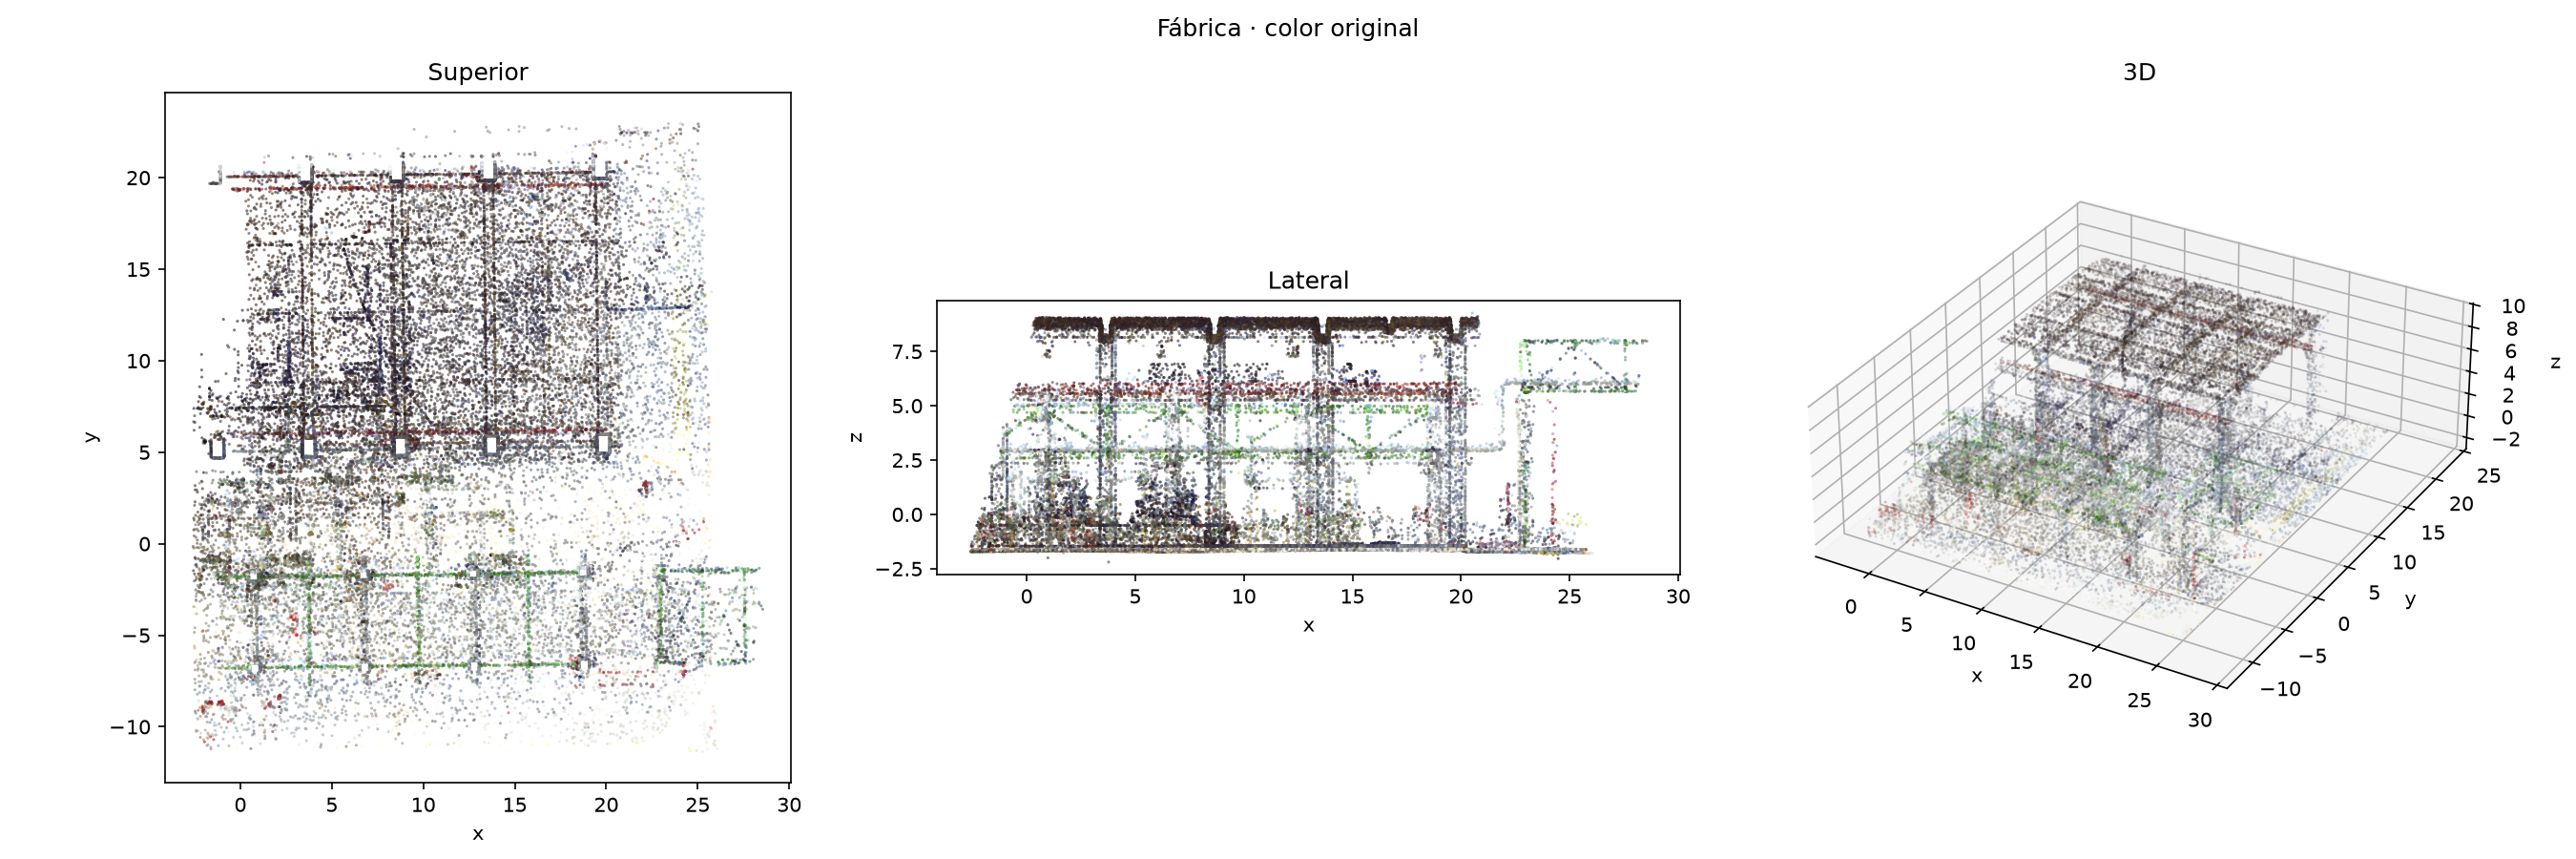
\includegraphics[width=\textwidth]{figs/01_original.png}
\caption{Nube original (submuestra) con su color. Vistas superior, lateral y 3D.}
\label{fig:original}
\end{figure}

Trabajar con 1.6 millones de puntos es lento en métodos como el clustering jerárquico, así
que usamos \textit{voxel downsampling}: dividimos el espacio en cubitos y nos quedamos con un
punto por cubito. Con un voxel de 0.187 m quedaron 93\,903 puntos. Todos los notebooks usan
esa misma muestra para poder comparar, y al final propagamos las etiquetas a los puntos
completos con el vecino más cercano.

\section{Preprocesamiento}
\textbf{Estandarización.} Las coordenadas están en metros (rango de decenas), las normales
entre $-1$ y $1$ y el color en Lab entre 0 y 100. Como k-means y PCA usan distancias, una
variable con escala grande domina a las demás, así que estandarizamos (media 0, desviación
1). Lo comprobamos con PCA (figura~\ref{fig:pca}): sin estandarizar, dos componentes
explican el 82.7\,\% de la varianza solo porque las coordenadas y el color tienen escalas
grandes; estandarizando bajan a 47.0\,\% y se necesitan 7 componentes para llegar al 90\,\%.

\textbf{Color.} Convertimos RGB a CIE Lab, porque en ese espacio la distancia euclidiana se
parece más a la diferencia de color que percibimos.

\textbf{Altura.} Agregamos \textit{height}, que es $z$ menos el percentil 1 de $z$, como
una forma de medir la altura sobre el piso.

\section{Metodología}

\subsection{Lo visto en clase}
\begin{itemize}
\item \textbf{k-means} \cite{lloyd1982}: elegimos $K$ centros, asignamos cada punto al centro
más cercano y movemos cada centro al promedio de sus puntos, repitiendo hasta que nadie
cambie. Depende de la inicialización y asume grupos más o menos redondos.
\item \textbf{DBSCAN} \cite{ester1996}: define grupos como regiones densas. Hay que elegir un
radio $\varepsilon$ y un mínimo de vecinos \textit{minPts}; los puntos aislados quedan como
ruido. No pide $K$.
\item \textbf{Clustering jerárquico aglomerativo}: parte con cada punto solo y va uniendo los
dos grupos más cercanos. El resultado cambia con el \textit{linkage} (single, complete,
average, Ward).
\item \textbf{Gaussian Mixture (GMM)}: modela los datos como una mezcla de gaussianas y la
ajusta con EM; el número de componentes se elige con BIC.
\item \textbf{PCA}: proyecta a las direcciones de mayor varianza. Lo usamos para entender las
variables, y t-SNE solo para visualizar.
\end{itemize}

\subsection{Métricas sin etiquetas}
Como no hay etiquetas reales usamos: el \textit{silhouette} \cite{rousseeuw1987} (qué tan bien
separado está cada punto de los otros grupos, entre $-1$ y 1, más alto es mejor), el índice de
Davies-Bouldin \cite{davies1979} (más bajo es mejor), el porcentaje de ruido, el tamaño del
grupo más grande y la estabilidad: repetir con otras semillas o submuestras y medir el
Adjusted Rand Index (ARI) \cite{hubert1985} entre corridas (1 significa mismas particiones).
Todo se calcula con scikit-learn \cite{pedregosa2011} y los valores de silhouette y
Davies-Bouldin comparables se miden sobre el mismo espacio de variables estandarizado.

\subsection{Mejora en etapas}
Los problemas de la línea base nos dieron la idea de las etapas (los detallamos en la
sección~\ref{sec:etapas}):
\begin{enumerate}
\item \textbf{Estructura (RANSAC)} \cite{fischler1981}: ajusta planos con muestras
aleatorias de puntos y se queda con el plano que más puntos explica. Usamos las normales para
decidir si un plano es horizontal ($|n_z|>0.9$) o vertical ($|n_z|<0.2$). Sirve para sacar el
piso y el techo.
\item \textbf{Orientación local}: para cada punto miramos sus $k=96$ vecinos y hacemos PCA
local. Los autovalores dan la \textit{linealidad} (parece una barra), la \textit{planaridad}
(parece una chapa) y la dirección principal. Con eso separamos los puntos en: lineal vertical
(columnas), lineal horizontal en $x$, lineal horizontal en $y$ y planar.
\item \textbf{Agrupar por distancia dentro de cada orientación} con HDBSCAN
\cite{campello2013}, que es como DBSCAN pero prueba varios radios y no necesita elegir
$\varepsilon$ (usamos \texttt{hdbscan} \cite{mcinnes2017}). Luego unimos fragmentos
colineales pequeños para no sobresegmentar.
\item \textbf{Clases heurísticas}: a cada grupo le ponemos un nombre con reglas
simples (por ejemplo, ``columna'' si es vertical, alargado y de más de 2 m de alto).
Son reglas que nosotros definimos, no un clasificador entrenado.
\end{enumerate}

\section{Diseño experimental}
Todo es no supervisado y con semilla fija (0). Probamos 128 configuraciones en la parte de
clase: 88 de k-means (4 combinaciones de variables, con y sin estandarizar, $K=2..12$), 10 de
DBSCAN (grilla de $\varepsilon$ y \textit{minPts}), 16 de clustering jerárquico y 14 de GMM.
Para elegir la configuración final de clase pedimos entre 6 y 15 grupos, máximo 30\,\% de
ruido y que ningún grupo tenga más del 60\,\% de los puntos, y entre las que cumplían
ordenamos por silhouette, Davies-Bouldin y ARI. Esta regla la cambiamos después de ver que
la primera versión (solo silhouette) elegía $K=2$ (ver sección~\ref{sec:clase}).

En la mejora en etapas hicimos ablaciones: quitar la separación por orientación, quitar las
normales, agregar color, cambiar el voxel (0.10, 0.15, 0.25 m), el $\varepsilon$ y
\textit{minPts}, y DBSCAN contra HDBSCAN. La estabilidad se midió con tres submuestras de voxel
distinto. El código y los notebooks se ejecutaron de punta a punta sin errores.

\section{Resultados}

\subsection{Lo visto en clase}\label{sec:clase}
\textbf{k-means.} El silhouette más alto lo obtuvieron configuraciones con $K=2$ (por ejemplo,
0.261 con todas las variables), que solo separan el techo del resto. Esto nos enseñó que el
silhouette favorece pocos grupos grandes y que no sirve por sí solo para decidir $K$
(figura~\ref{fig:kmeans}). Con la regla de 6--15 grupos quedó $K=11$ con $xyz$ + color Lab +
normales + altura, estandarizado: silhouette común 0.213, Davies-Bouldin 1.51, ARI entre
semillas 0.95 y el grupo más grande con 20.4\,\% de los puntos.

\begin{figure}[!htb]
\centering
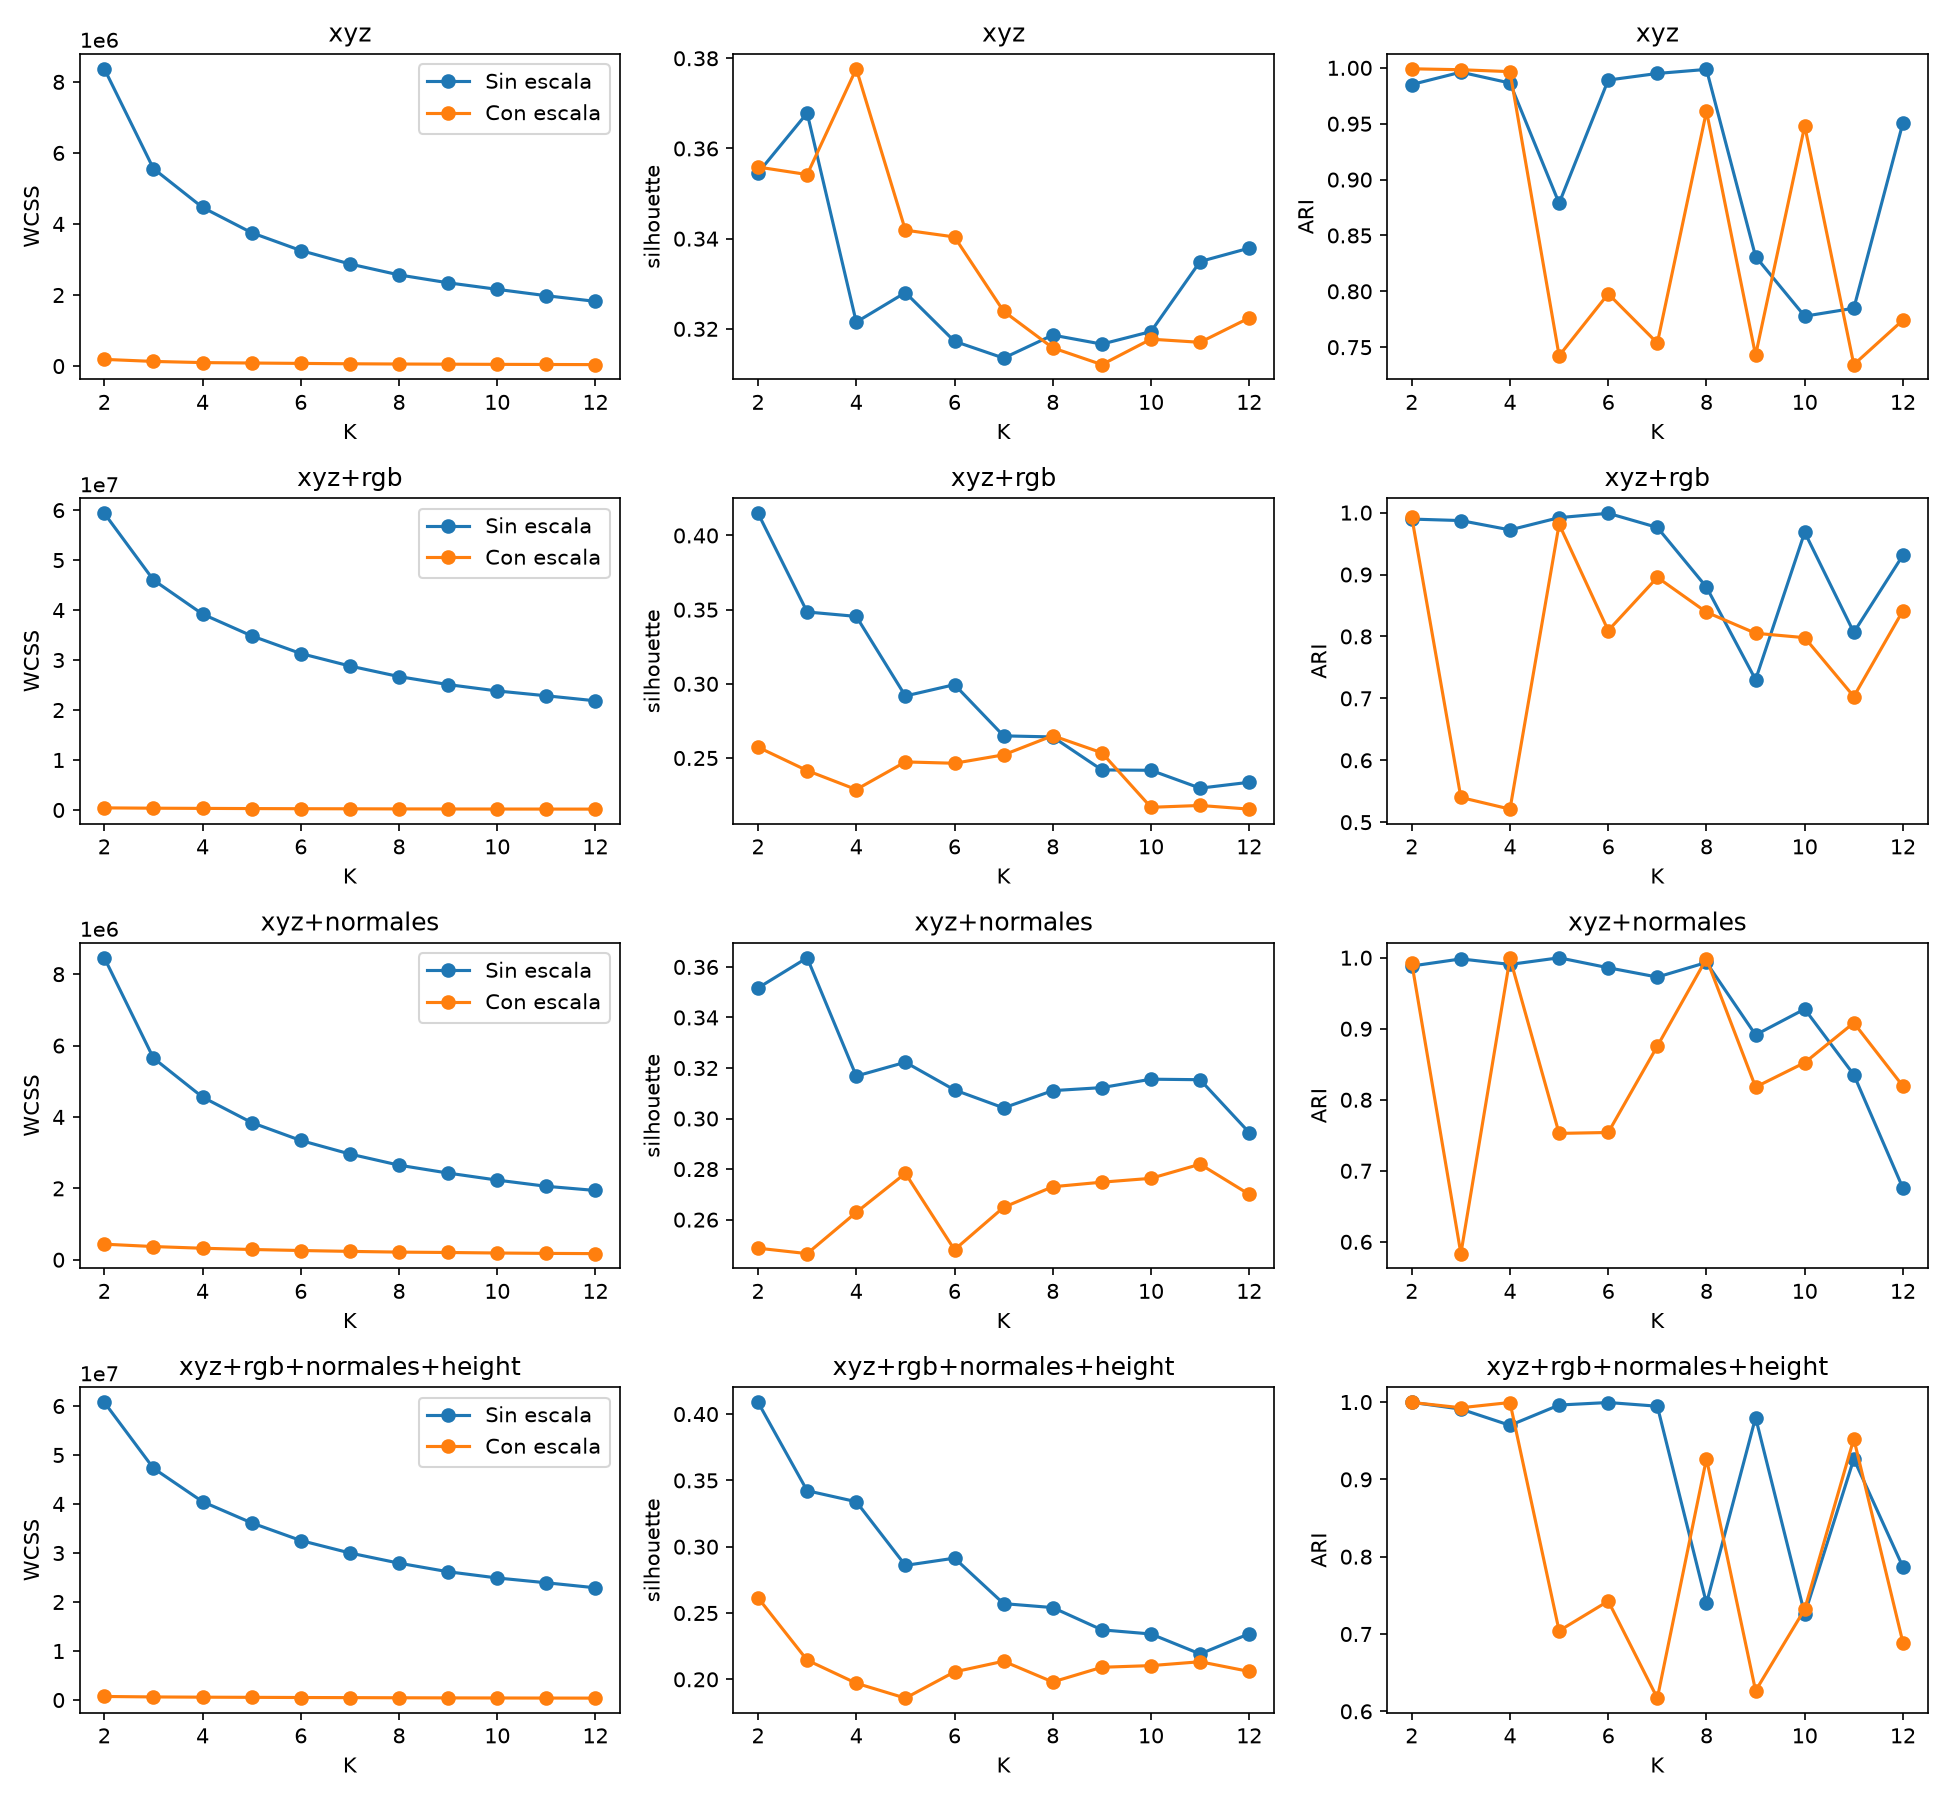
\includegraphics[width=0.9\textwidth]{figs/02_curvas.png}
\caption{k-means: curva del codo (WCSS) y silhouette para $K=2,\dots,12$ con distintas variables.}
\label{fig:kmeans}
\end{figure}

\textbf{DBSCAN.} Elegimos $\varepsilon$ con la curva de distancia al $k$-ésimo vecino
(figura~\ref{fig:kdist}). Con $\varepsilon$ muy chico casi todo es ruido (99.9\,\%, aunque el
silhouette se ve alto porque solo se calcula sobre lo que no es ruido). Con $\varepsilon\approx0.11$
casi todo (99.2\,\%) cae en un solo grupo. En esta nube, la estructura está tan conectada que
DBSCAN solo tiene dos comportamientos: todo pegado o todo ruido.

\begin{figure}[!htb]
\centering
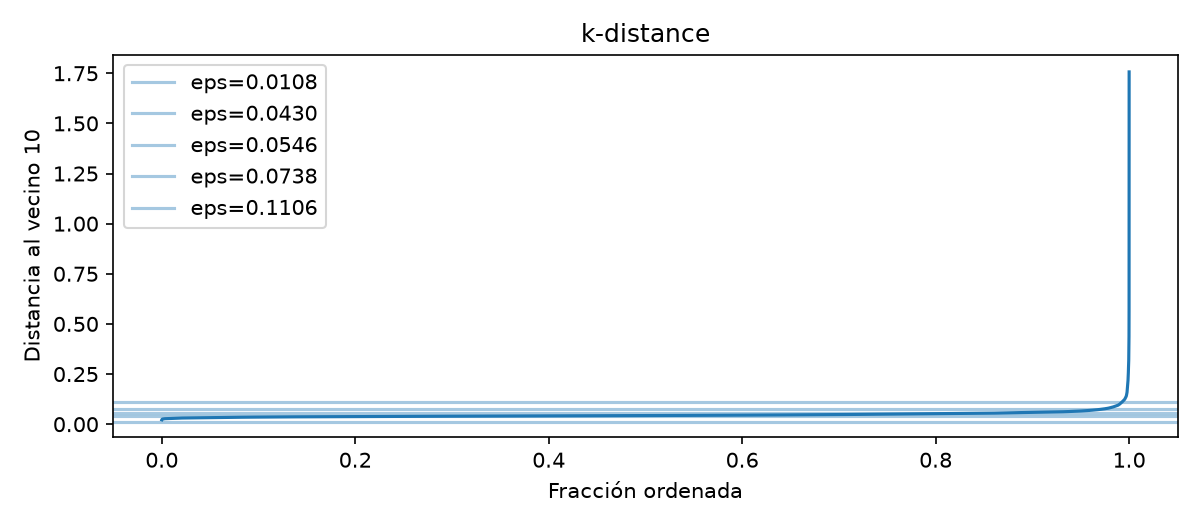
\includegraphics[width=0.6\textwidth]{figs/03_kdistance.png}
\caption{Curva de distancia al $k$-ésimo vecino para elegir $\varepsilon$ en DBSCAN.}
\label{fig:kdist}
\end{figure}

\textbf{Jerárquico y GMM.} Los mejores silhouette de ambos también fueron con 2 grupos (0.255
para average con $K=2$; 0.260 para GMM diagonal con 2 componentes). El BIC prefirió modelos
con más componentes dentro del rango probado, pero con silhouette bajo (0.066 con 8
componentes). La figura~\ref{fig:comp} resume la comparación.

\begin{figure}[!htb]
\centering
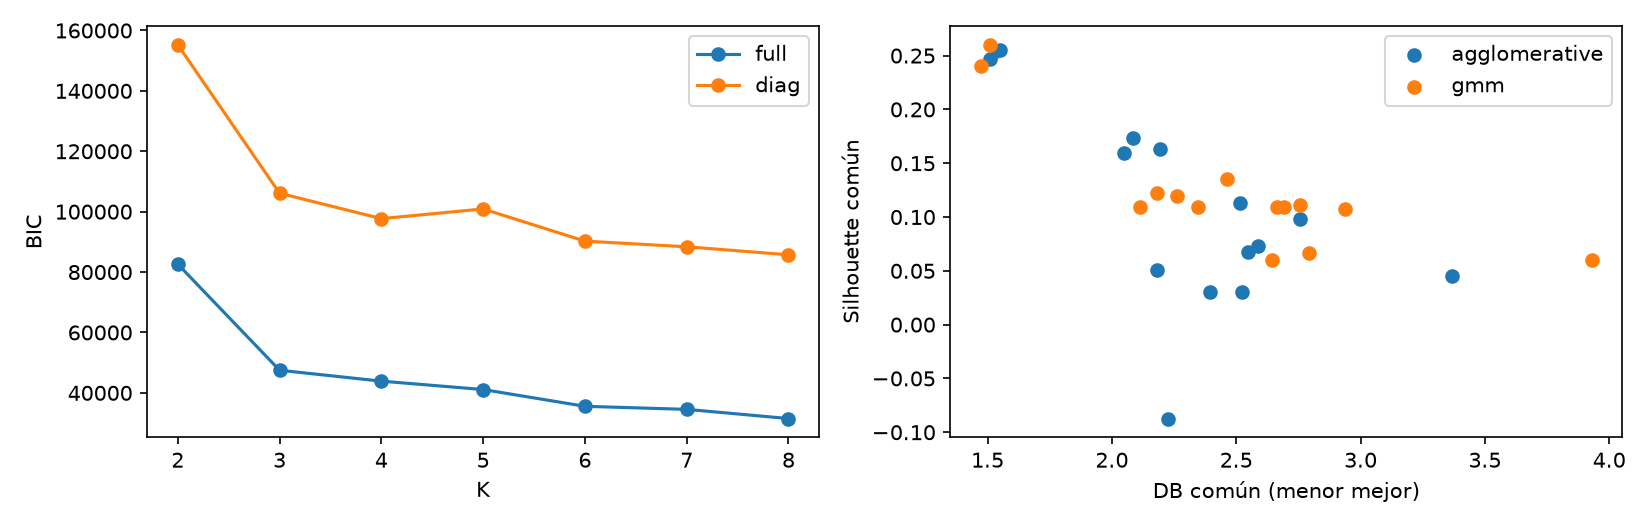
\includegraphics[width=0.9\textwidth]{figs/04_comparacion.png}
\caption{Comparación de jerárquico y GMM en silhouette y Davies-Bouldin.}
\label{fig:comp}
\end{figure}

\textbf{PCA y visualización.} La figura~\ref{fig:pca} muestra proyecciones de las variables
(PCA y t-SNE sobre una muestra pequeña, solo para mirar). Sirvieron para ver que hay grupos
reales, pero no para segmentar, porque t-SNE no conserva distancias globales.

\begin{figure}[!htb]
\centering
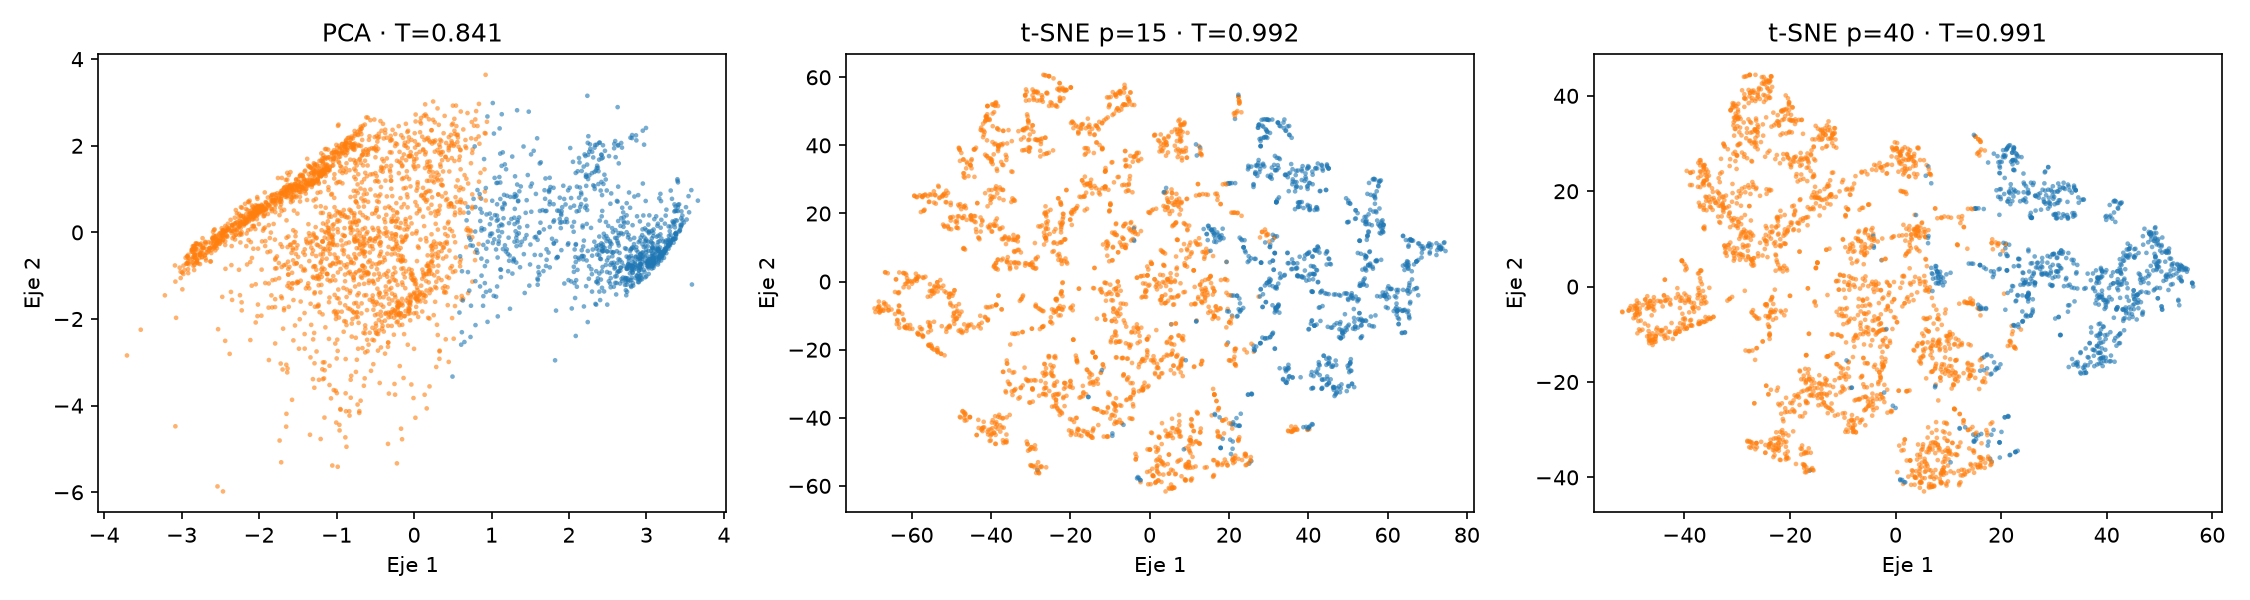
\includegraphics[width=0.9\textwidth]{figs/05_mapas.png}
\caption{Proyecciones PCA y t-SNE de las variables, coloreadas por cluster de k-means.}
\label{fig:pca}
\end{figure}

\textbf{Resultado de clase.} La figura~\ref{fig:clasefinal} muestra el k-means $K=11$
propagado a toda la nube y la figura~\ref{fig:clasepaneles} cada grupo por separado. Se
distinguen el techo (grupo 0), un tramo de vigas con forma de celosía (grupo 4), una tubería
horizontal larga (grupo 5) y columnas (grupos 3 y 7). Pero el piso quedó repartido en tres
grupos (1, 2 y 8) y solo 36\,\% del piso quedó en su grupo más grande (10 grupos tocan el
piso), y hay grupos mezcla de equipos bajos y estructura. Además no distingue cada columna
como un objeto aparte.

\begin{figure}[!htb]
\centering
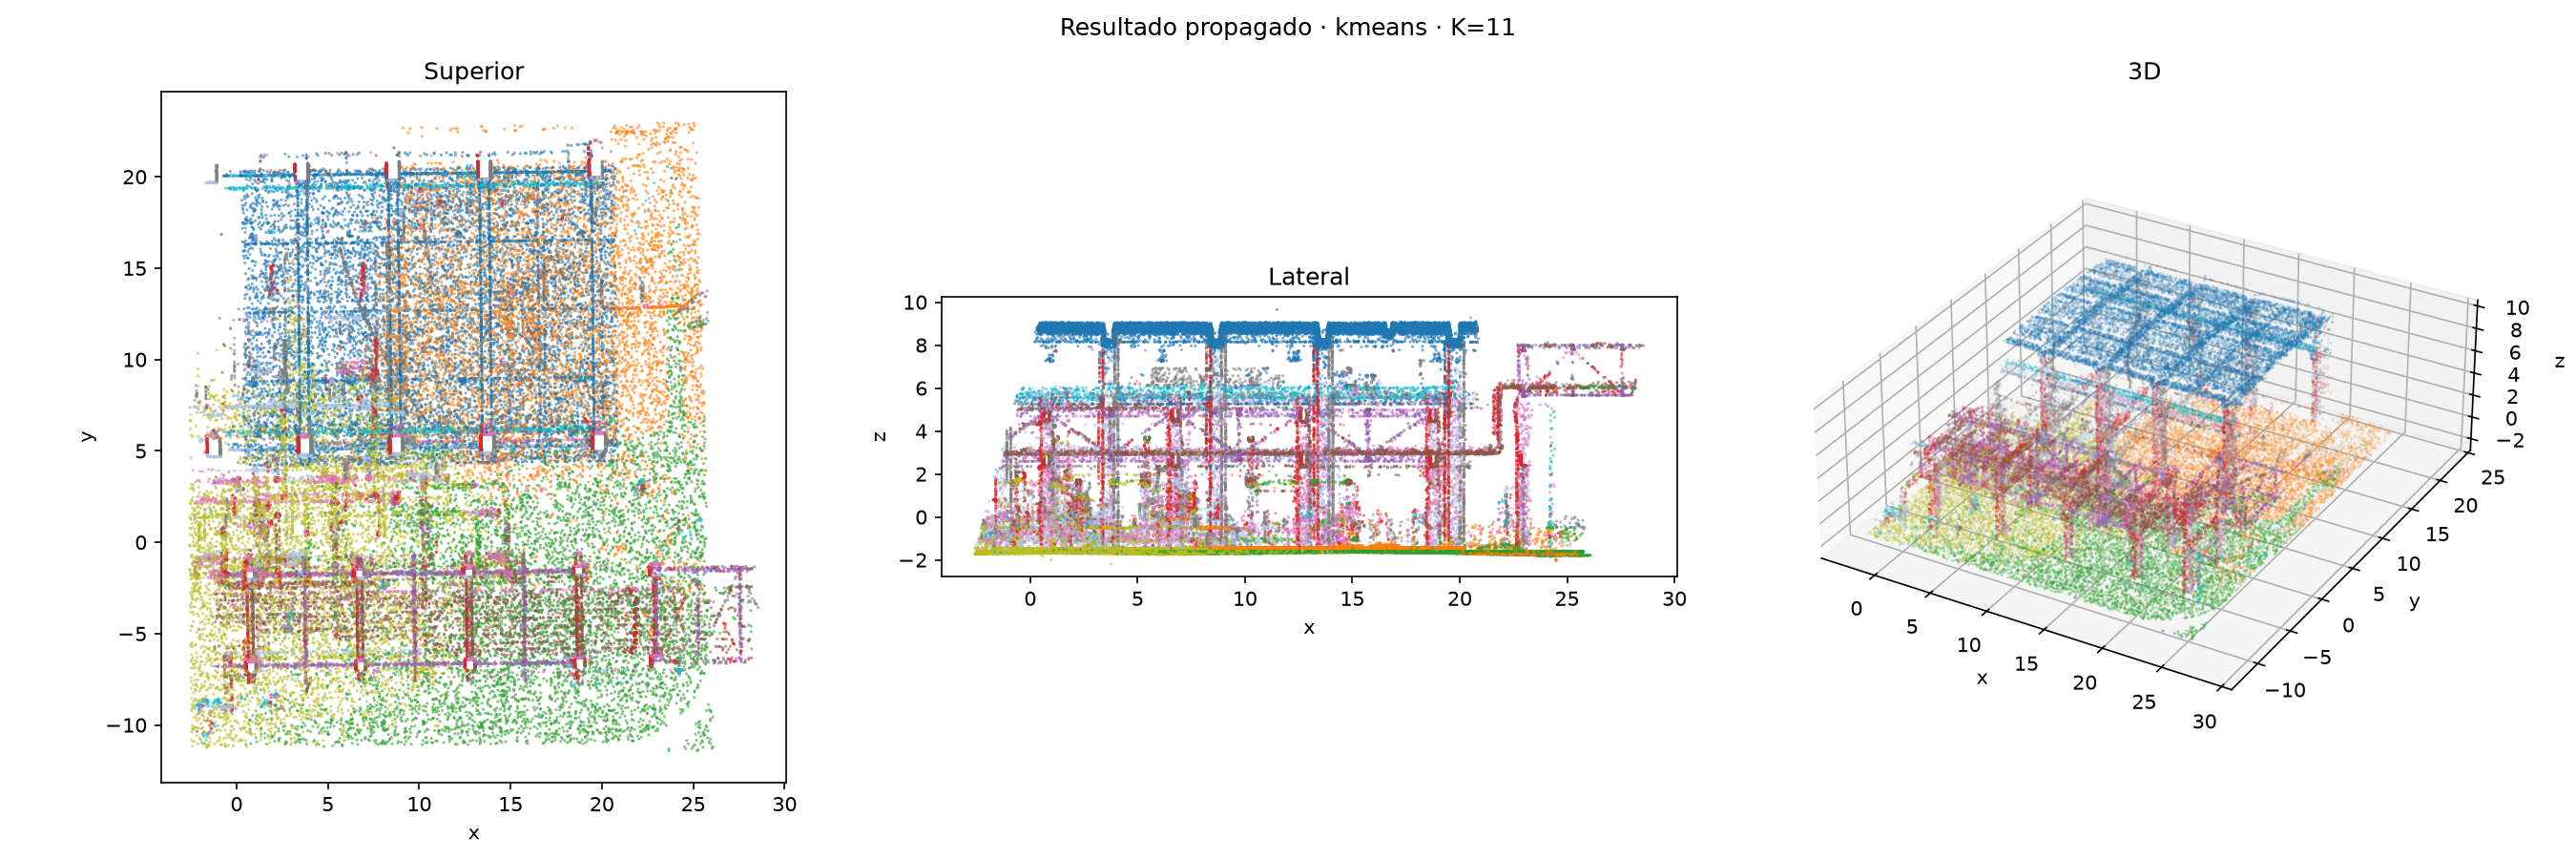
\includegraphics[width=\textwidth]{figs/06_completo.png}
\caption{Resultado de clase: k-means $K=11$ propagado a los 1\,647\,021 puntos.}
\label{fig:clasefinal}
\end{figure}

\begin{figure}[!htb]
\centering
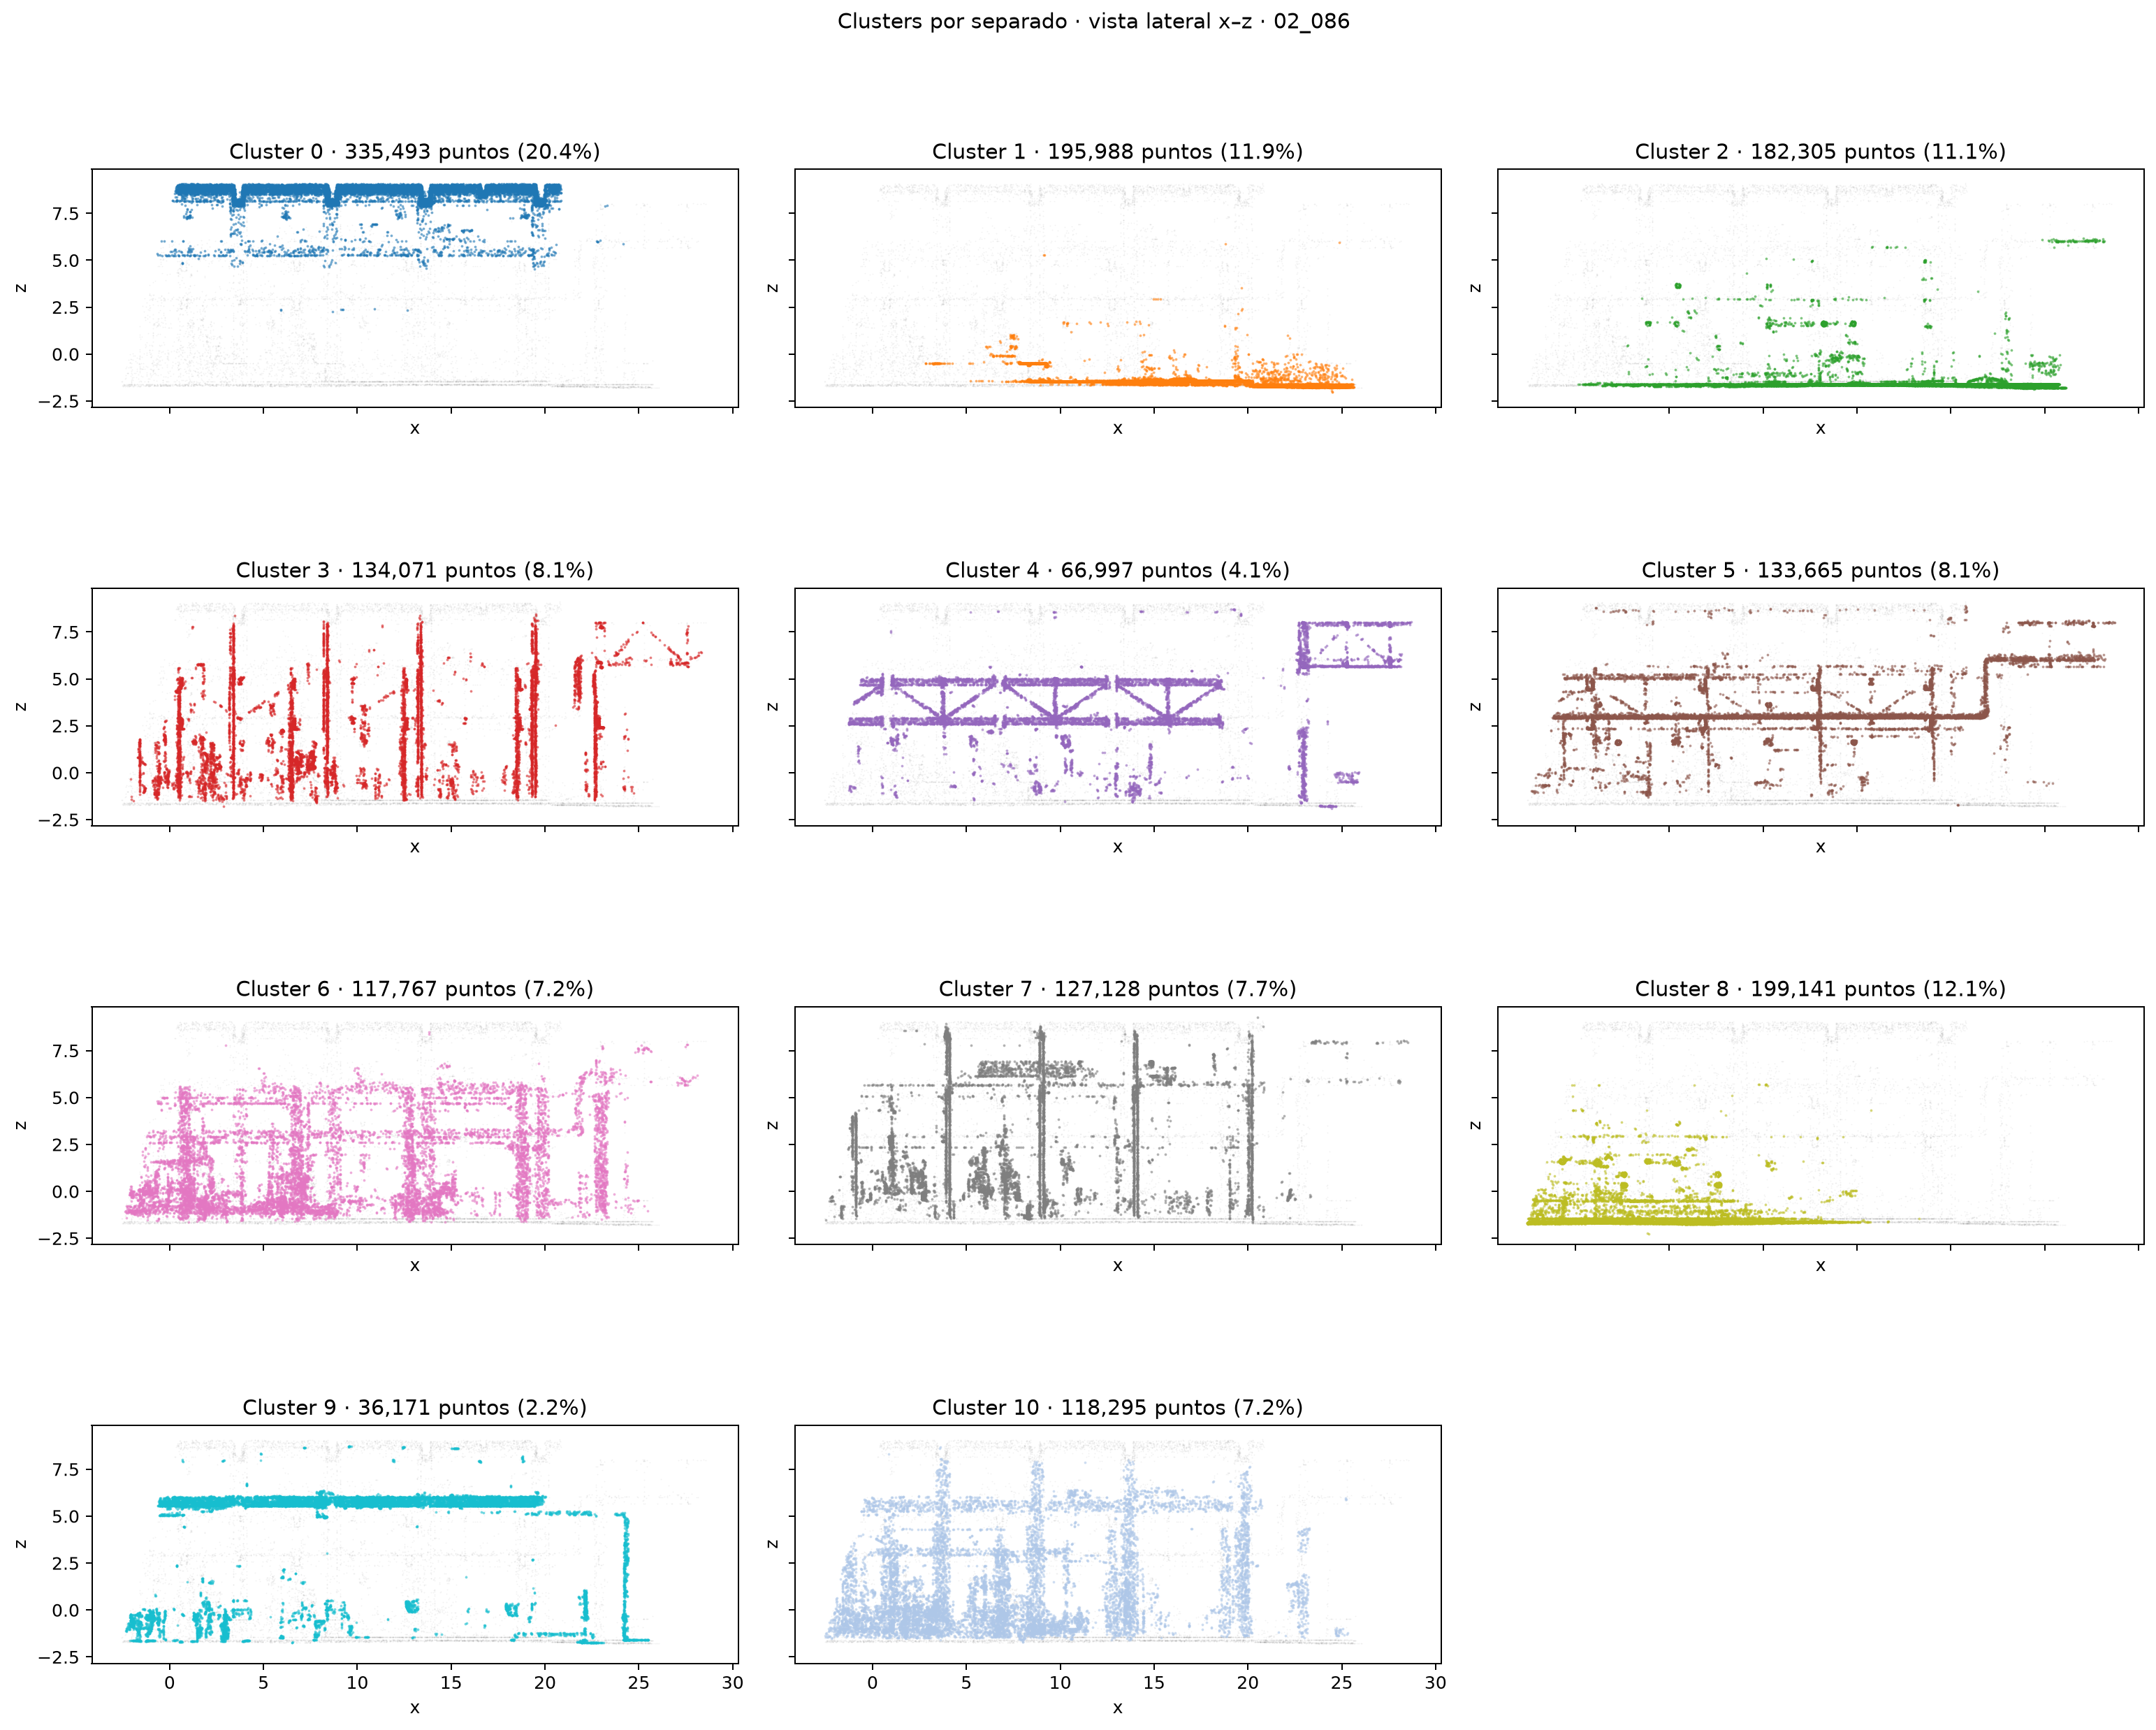
\includegraphics[width=\textwidth]{figs/06_clusters_separados.png}
\caption{Cada grupo de k-means por separado (vista lateral $x$--$z$); los puntos grises son el resto de la nube.}
\label{fig:clasepaneles}
\end{figure}
\FloatBarrier

\subsection{Mejora en etapas}\label{sec:etapas}
\textbf{Etapa 1: piso y techo.} RANSAC encontró dos planos grandes, el piso con 488\,252
puntos (29.6\,\%) y el techo con 111\,522 (6.8\,\%). Con un umbral de 0.08 m el piso queda
completo en un solo segmento (con 0.03 m solo un 80\,\% de los puntos del piso). La figura~\ref{fig:etapa1} lo
muestra. Los supuestos planos verticales (paredes) se descartaron porque cubrían solo 12--18\,\%
de su rectángulo, menos que el 55\,\% que exigimos, y en realidad eran estructura metálica.

\begin{figure}[!htb]
\centering
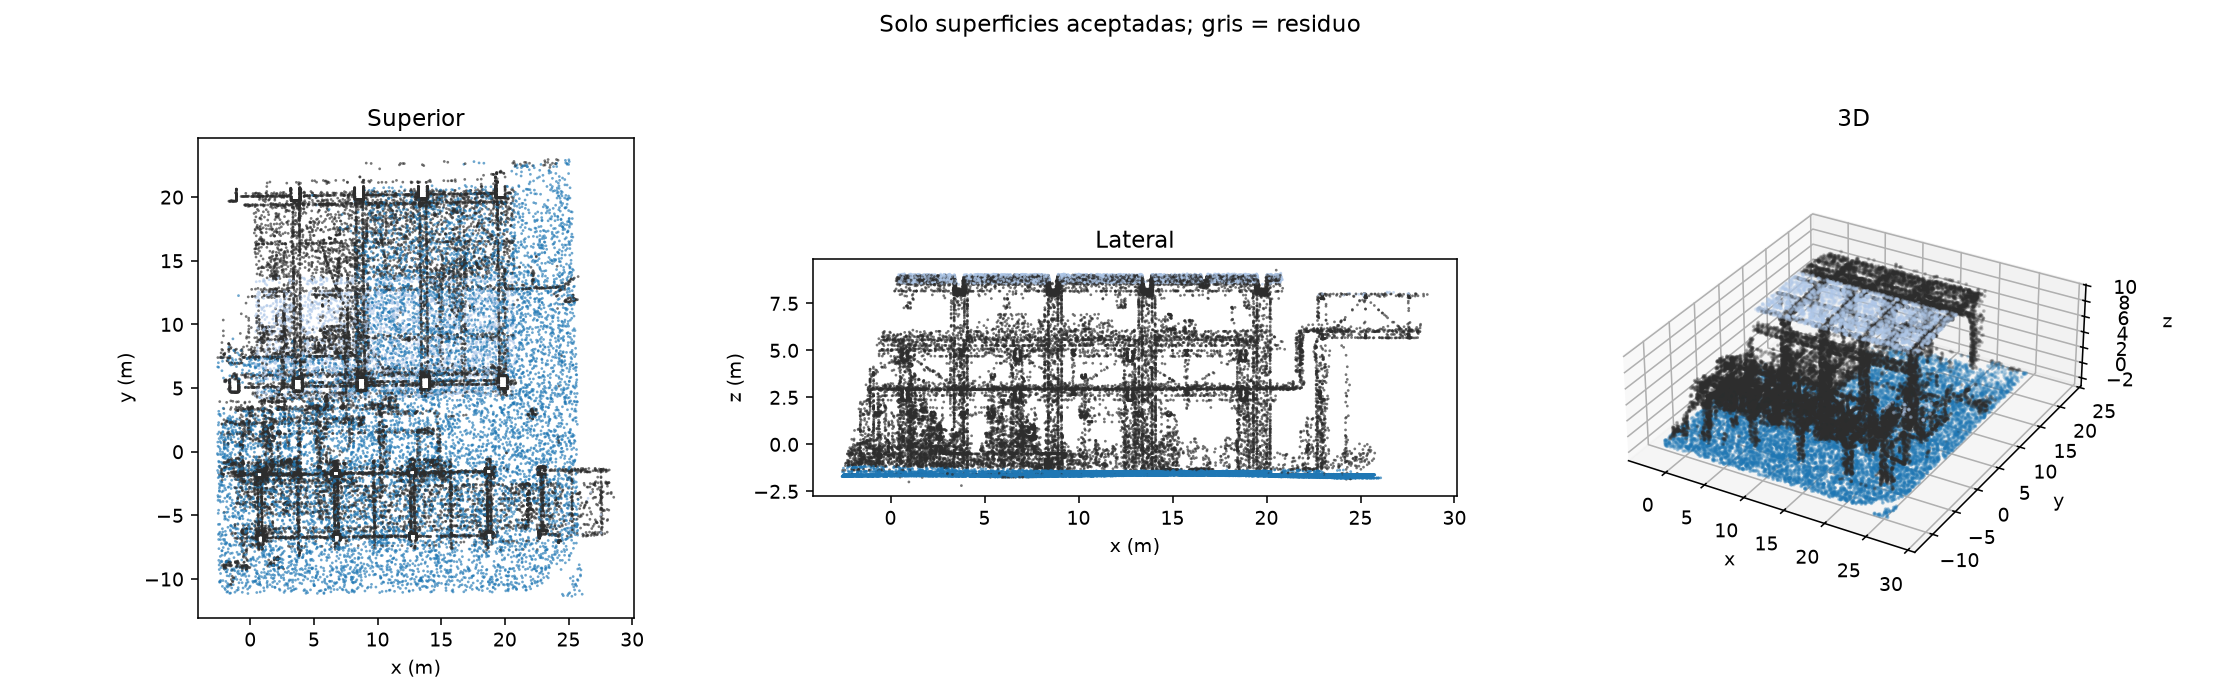
\includegraphics[width=\textwidth]{figs/exp_01_estructura.png}
\caption{Etapa 1: piso y techo extraídos con RANSAC.}
\label{fig:etapa1}
\end{figure}

\textbf{Etapa 2: orientación antes que distancia.} Al correr DBSCAN directo sobre lo que
queda, casi toda la estructura (61\,\%) terminaba como una sola componente conexa. Al separar
antes por orientación local (figura~\ref{fig:orient}) y agrupar dentro de cada clase, la
mezcla bajó de 61.1\,\% a 7.6\,\% con DBSCAN y a 15.5\,\% con HDBSCAN, y los grupos de
columnas altas pasaron de 1 a 9--16 (tabla~\ref{tab:ablacion}).

\begin{figure}[!htb]
\centering
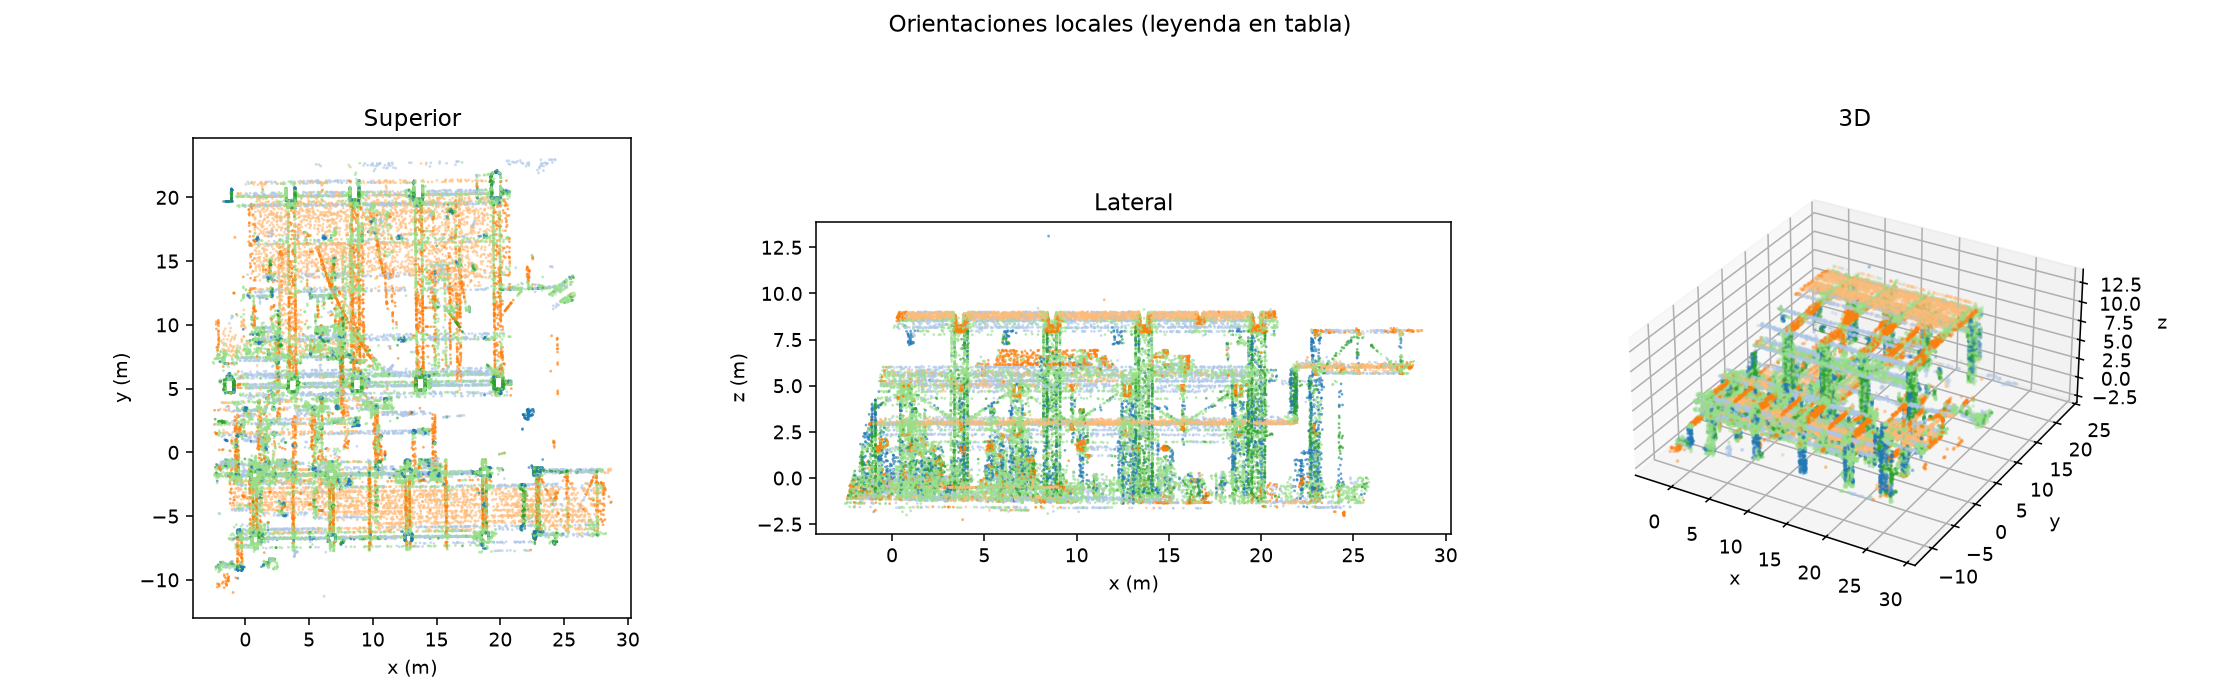
\includegraphics[width=\textwidth]{figs/exp_02_orientaciones.png}
\caption{Etapa 2: clases de orientación local (vertical, horizontal en $x$, horizontal en $y$, planar).}
\label{fig:orient}
\end{figure}

\textbf{Resultado final.} Nos quedamos con HDBSCAN por orientación (voxel 0.15 m, tamaño
mínimo de grupo 40), que dio 239 segmentos y 0.55\,\% de ruido. La tabla~\ref{tab:clases}
muestra el reparto por clase y la figura~\ref{fig:final} el resultado completo. La
figura~\ref{fig:panel} muestra cada clase por separado y la figura~\ref{fig:col} las
instancias de columna, con un color por instancia.

\begin{table}[!htb]
\centering
\caption{Reparto de la nube final por clase heurística.}
\label{tab:clases}
\begin{tabular}{lrrr}
\toprule
Clase & Segmentos & Puntos & \% \\
\midrule
Piso & 1 & 488\,252 & 29.64 \\
Viga horizontal & 53 & 319\,174 & 19.38 \\
Viga o tubería & 76 & 309\,460 & 18.79 \\
Mezcla no identificada & 63 & 256\,084 & 15.55 \\
Columna & 17 & 113\,352 & 6.88 \\
Techo & 1 & 111\,522 & 6.77 \\
Equipo bajo & 22 & 33\,860 & 2.06 \\
Compacto plausible & 6 & 6\,202 & 0.38 \\
Ruido & 1 & 9\,115 & 0.55 \\
\bottomrule
\end{tabular}
\end{table}

\begin{figure}[!htb]
\centering
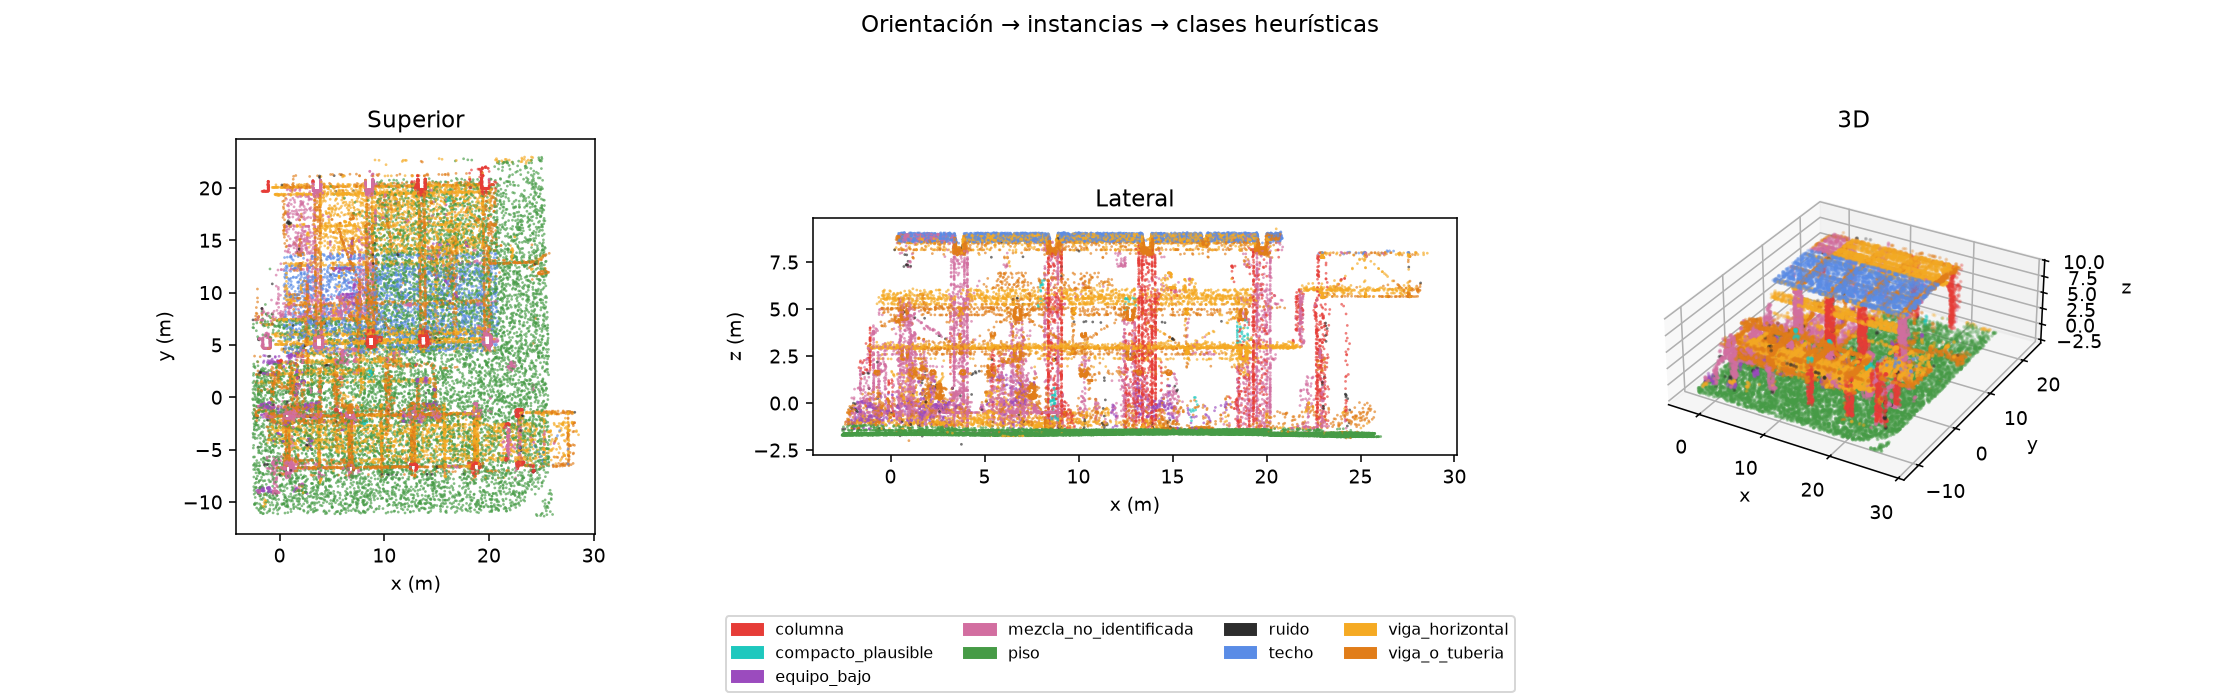
\includegraphics[width=\textwidth]{figs/exp_05_final.png}
\caption{Resultado final por etapas, con las clases heurísticas.}
\label{fig:final}
\end{figure}

\begin{figure}[!htb]
\centering
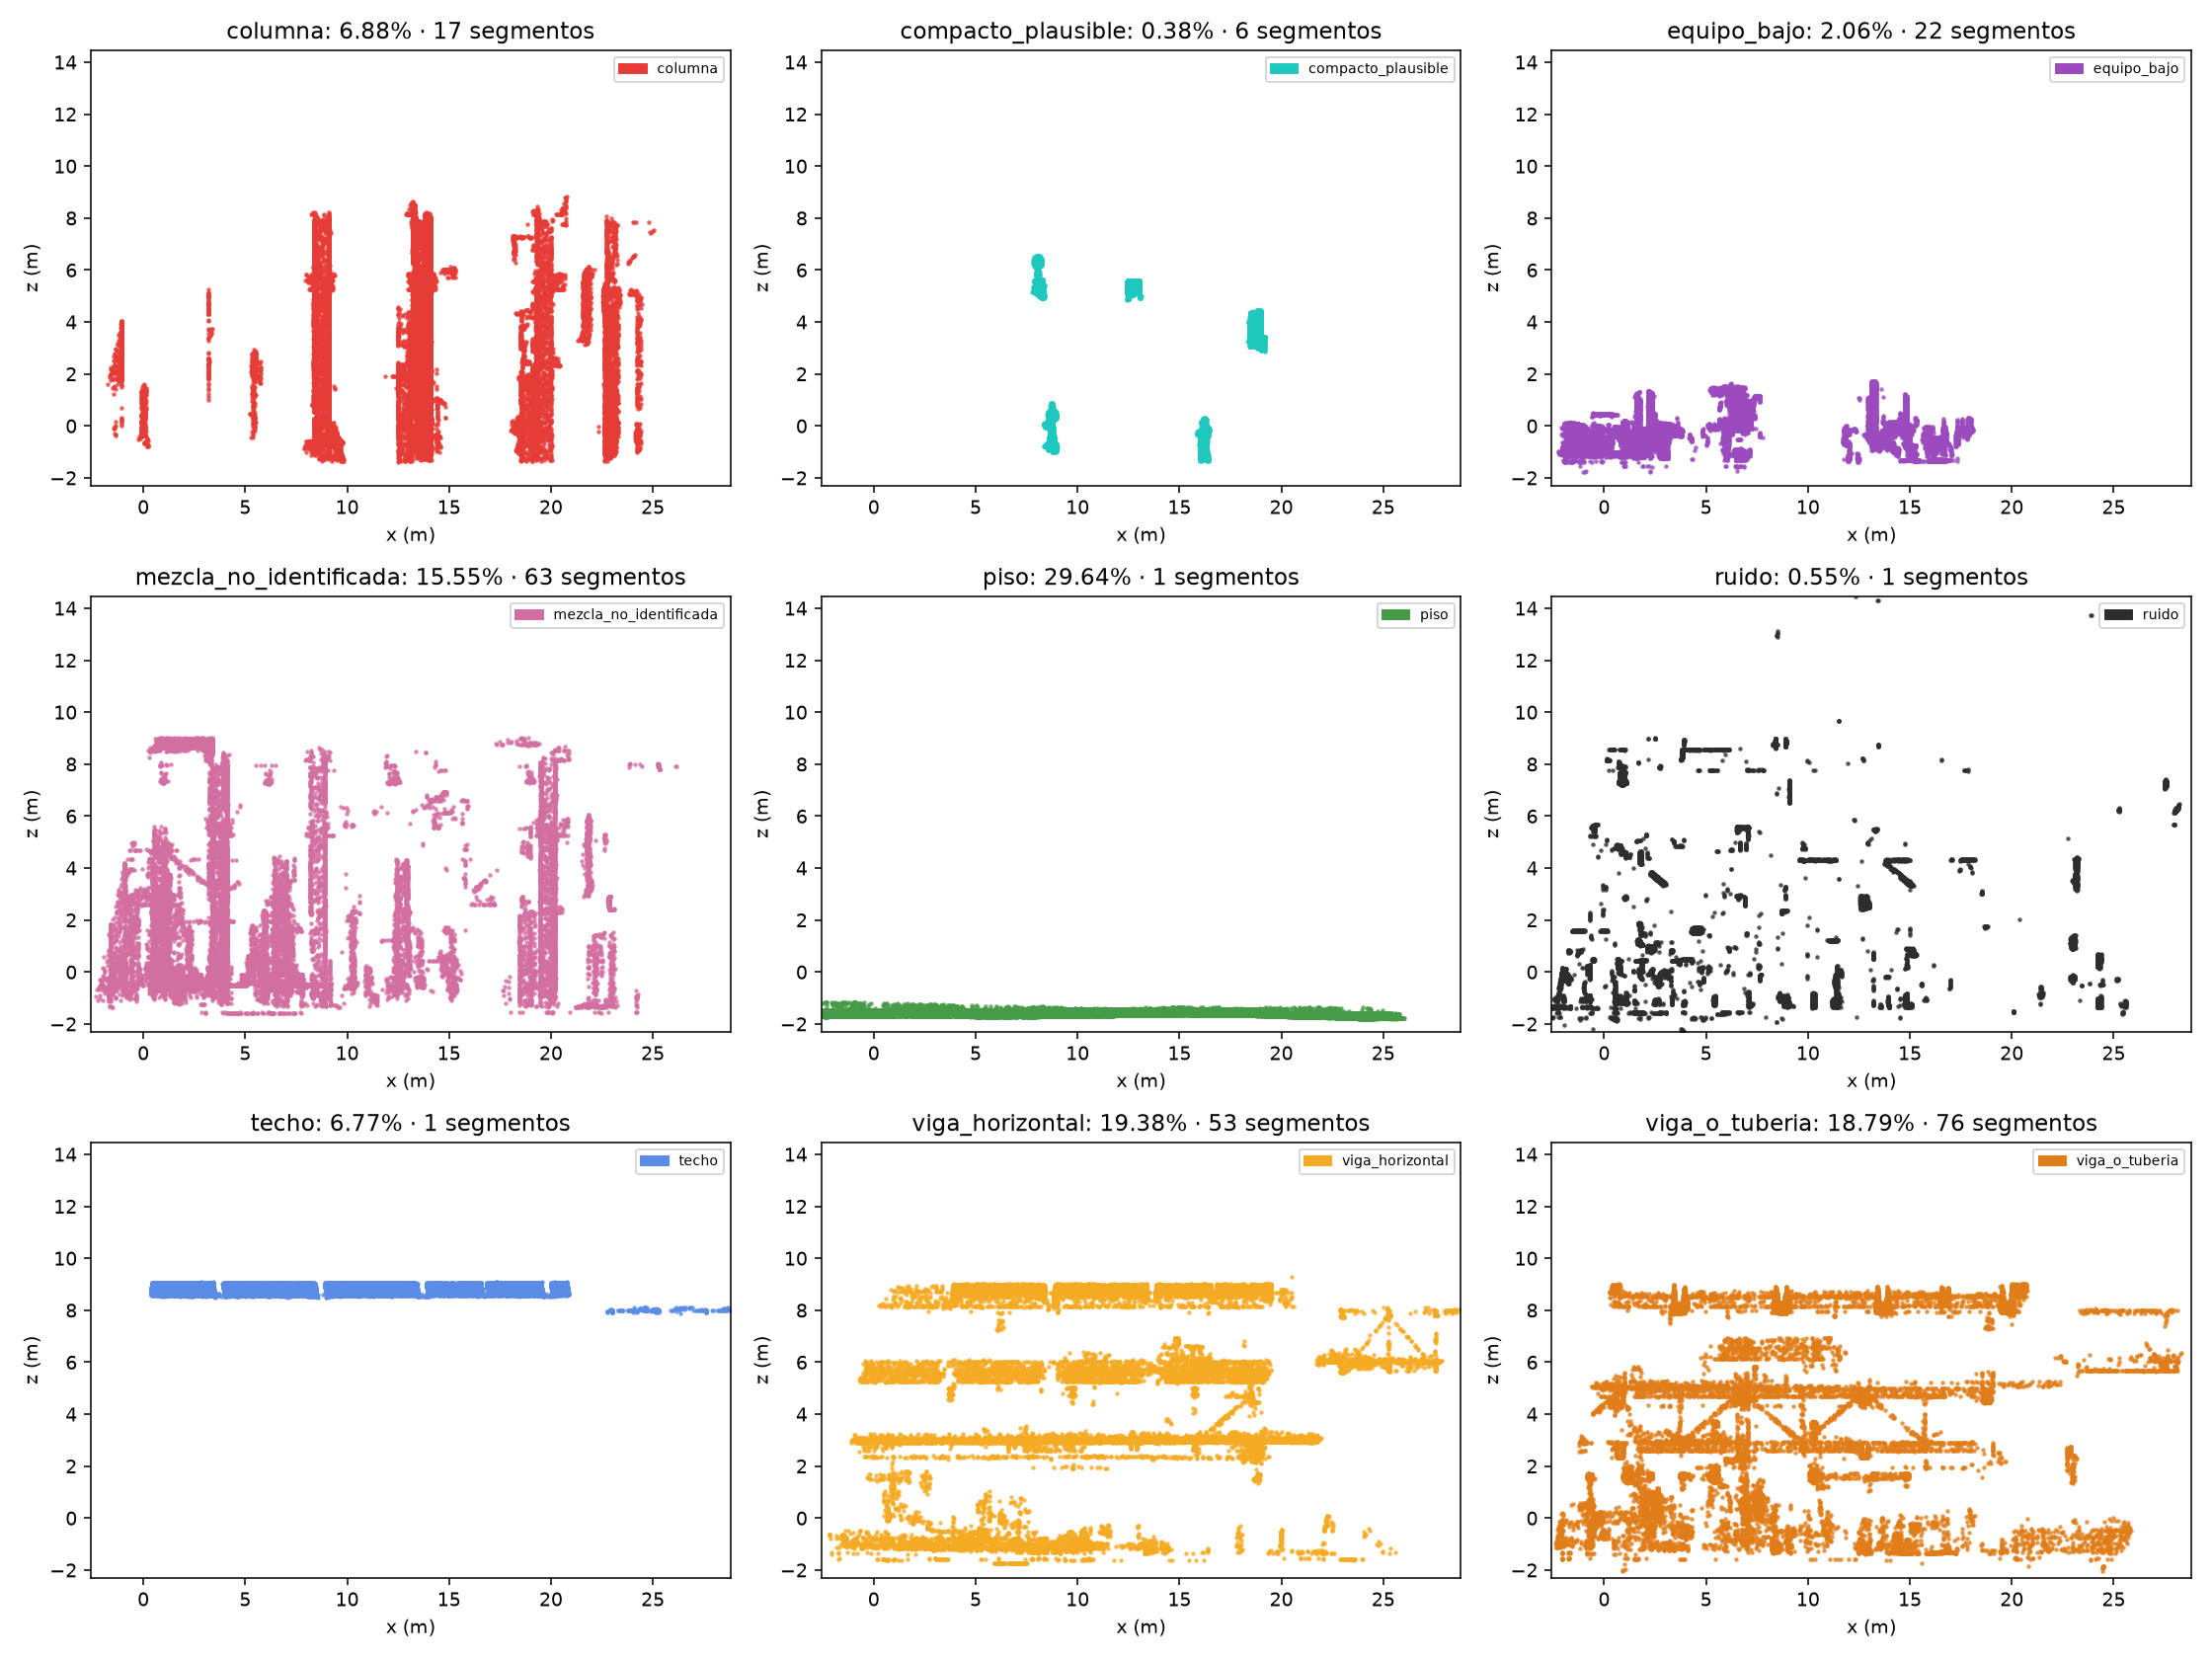
\includegraphics[width=0.95\textwidth]{figs/exp_05_panel_clases.png}
\caption{Cada clase heurística por separado (vista lateral).}
\label{fig:panel}
\end{figure}

\begin{figure}[!htb]
\centering
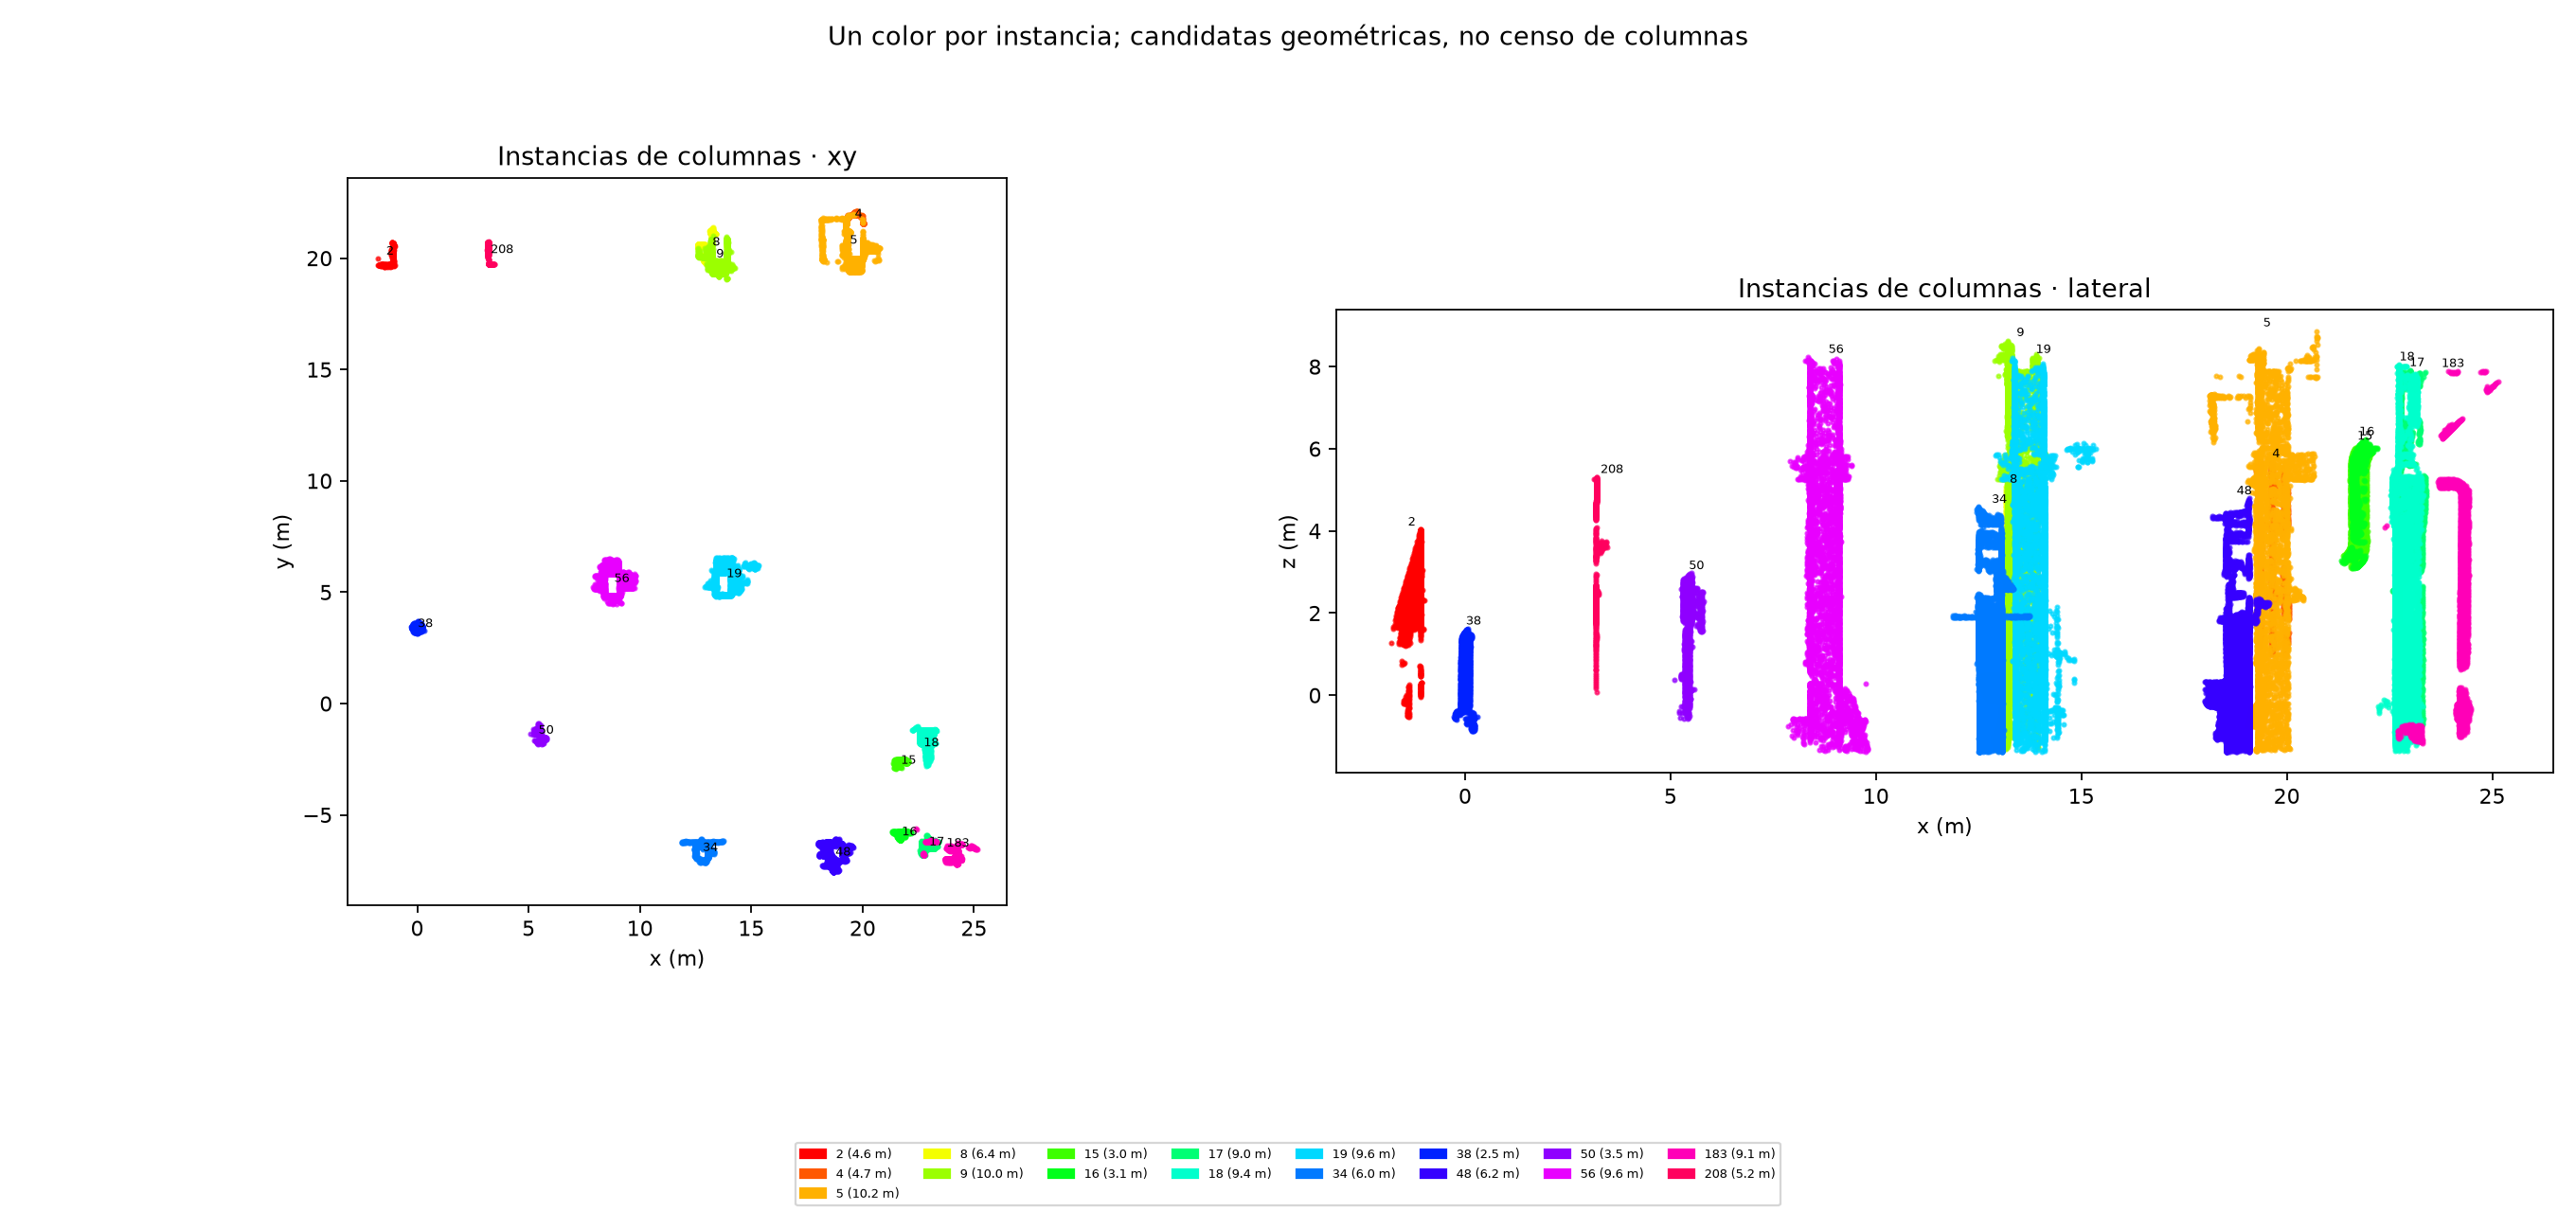
\includegraphics[width=\textwidth]{figs/exp_05_columnas_instancias.png}
\caption{Instancias de columna candidatas, un color por instancia (vistas superior y lateral).}
\label{fig:col}
\end{figure}

\textbf{Ablaciones.} La tabla~\ref{tab:ablacion} compara la línea base con variantes.
Sacar las normales hizo bajar la estabilidad de 0.97 a 0.55 (ARI), así que las normales
fueron lo más útil. Agregar color o altura casi no cambió nada, y el tamaño del voxel
modificó la cantidad de segmentos y de ruido (voxel de 0.25 m: 2.5\,\% de ruido). En el
control sin orientación se ve el problema original: un segmento que concentra 61\,\% de los
puntos. La figura~\ref{fig:abl} resume las ablaciones.

\begin{table}[!htb]
\centering
\caption{Ablaciones principales. Mezcla y columnas altas son sobre la nube completa; ARI es estabilidad entre submuestras (la línea base usa semillas, protocolo distinto).}
\label{tab:ablacion}
\small
\begin{tabular}{lrrrr}
\toprule
Configuración & Segmentos & Mezcla \% & Col. altas & ARI \\
\midrule
Línea base (k-means $K=11$) & 11 & --- & --- & 0.95 \\
DBSCAN sin orientación & 106 & 61.1 & 1 & 0.97 \\
DBSCAN con orientación & 664 & 7.6 & 16 & 0.97 \\
Con orientación sin normales & 708 & 7.6 & 16 & 0.55 \\
HDBSCAN (mín. 100) & 122 & 20.5 & 5 & 0.94 \\
\textbf{HDBSCAN (mín. 40, final)} & \textbf{239} & \textbf{15.5} & \textbf{9} & \textbf{0.97} \\
\bottomrule
\end{tabular}
\end{table}

\begin{figure}[!htb]
\centering
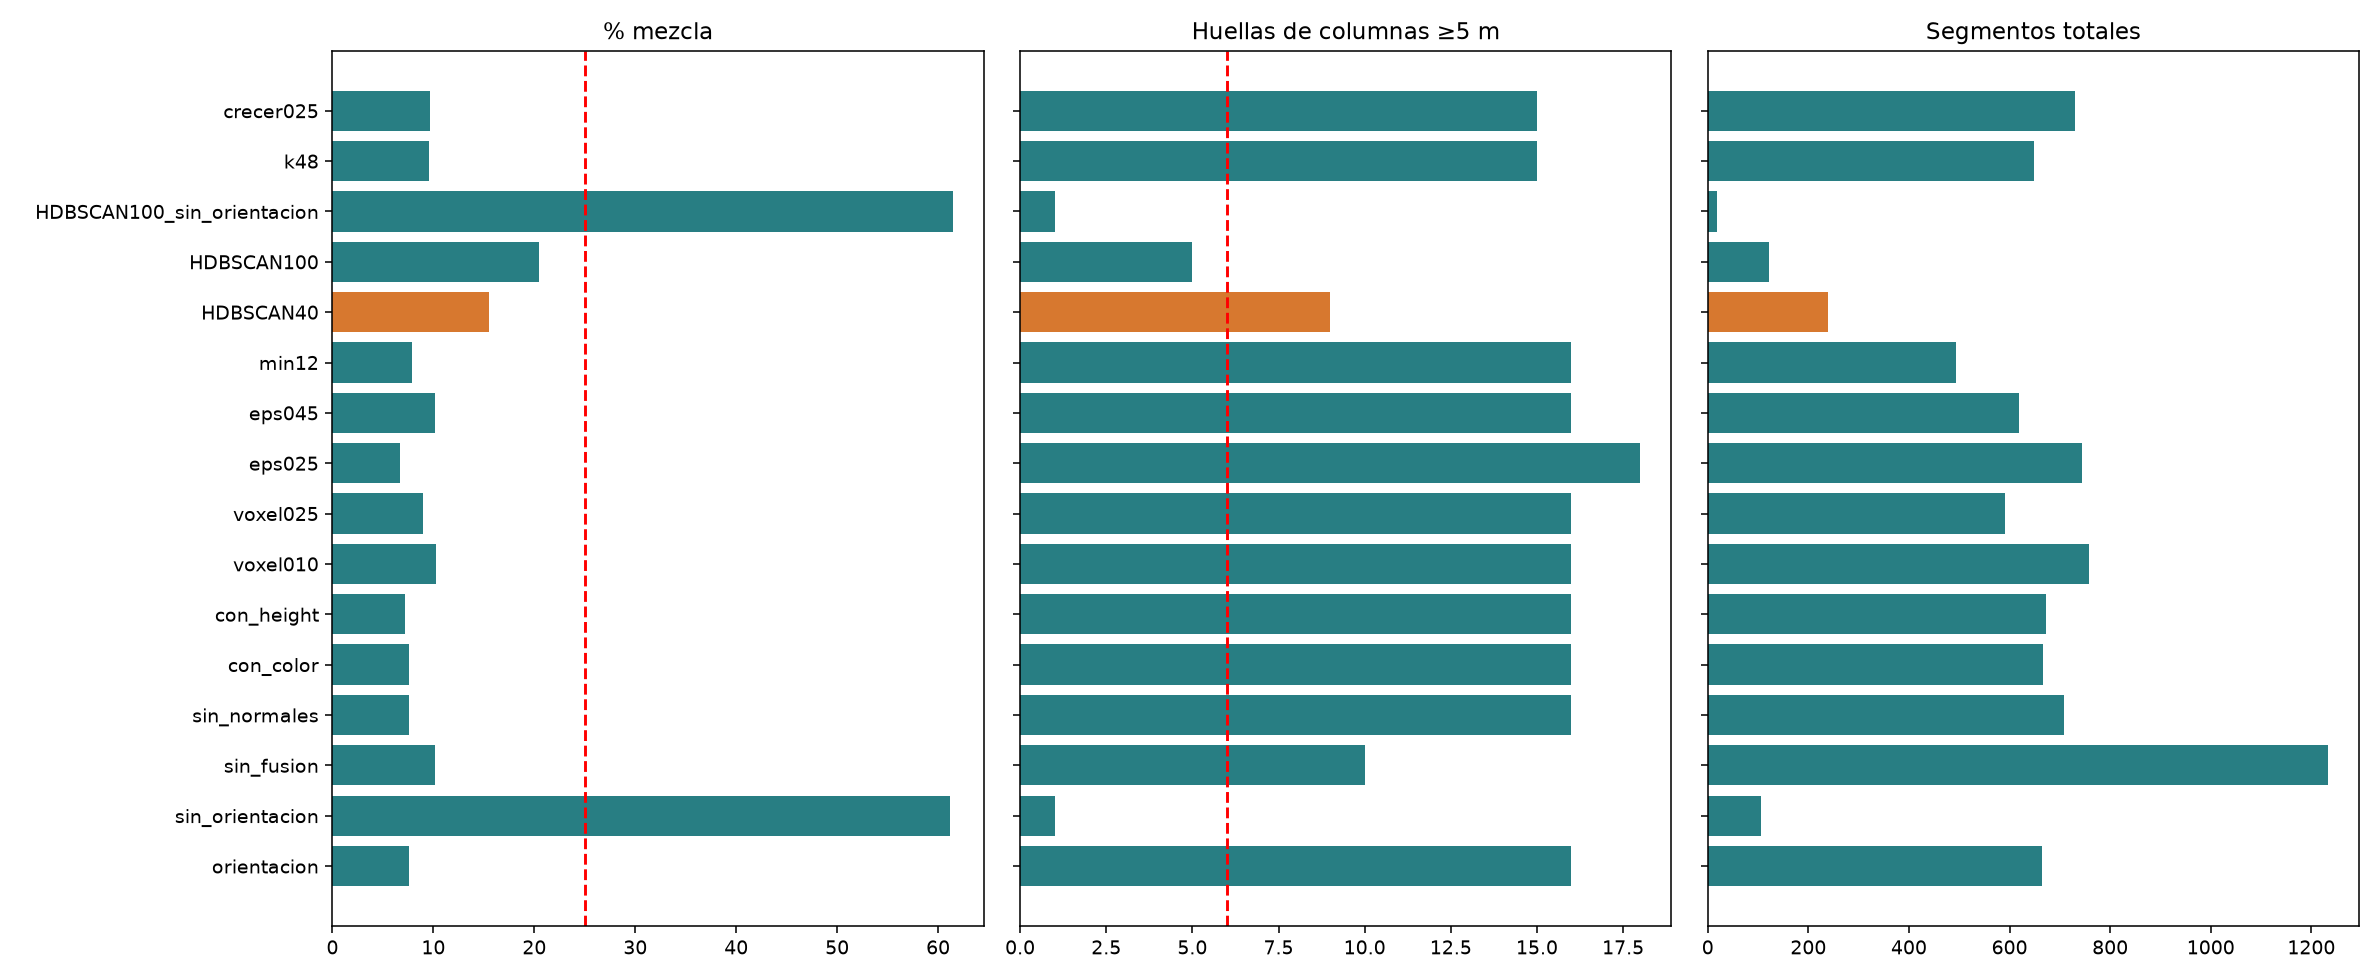
\includegraphics[width=0.85\textwidth]{figs/exp_04_resumen.png}
\caption{Resumen de las ablaciones.}
\label{fig:abl}
\end{figure}
\FloatBarrier

\textbf{Comparación justa con la línea base.} Comparar silhouette entre 11 y 239
segmentos no es justo, porque este índice premia pocos grupos. Por eso recalculamos las
métricas en las mismas variables geométricas, con 91\,981 puntos y colapsando a $K=11$: la
línea base obtuvo silhouette 0.146 y Davies-Bouldin 2.54 y el resultado final 0.107 y 2.59.
\textbf{Por lo tanto, el método en etapas no mejora las métricas internas}; su ventaja está en
cosas que esas métricas no miden: el piso es un solo segmento, se separan instancias de
columnas y las clases tienen un significado geométrico. La concordancia entre ambos
resultados es baja (ARI 0.17, NMI 0.26), lo que solo indica que son particiones distintas.

\section{Discusión y limitaciones}
\begin{itemize}
\item \textbf{No hay etiquetas reales.} No podemos decir qué porcentaje de puntos está bien
clasificado. Nuestra evaluación es interna, de estabilidad y visual, así que los números
sirven para comparar configuraciones y no para afirmar exactitud.
\item \textbf{Regla de selección cambiada.} Dos veces ajustamos la regla de selección después
de mirar los resultados: en clase (el silhouette elegía $K=2$) y en la etapa final (la
primera elegida omitía columnas que se veían claras en la vista lateral, por lo que exigimos
al menos 6 grupos de huellas altas). Es razonable, pero no es una elección fijada de
antemano, y lo declaramos por eso.
\item \textbf{Las clases son heurísticas.} Con linealidad y planaridad no pudimos distinguir
tuberías de vigas, así que quedó una clase ``viga o tubería''. Tampoco hay una clase
``truss'' ni ``pared'' confirmada. Los 6 grupos ``compactos plausibles'' no permiten decir
que haya personas o vehículos; no encontramos evidencia de ninguno.
\item \textbf{Columnas.} Los 17 segmentos de columna incluyen fragmentos y algunos soportes
que no son columnas completas (por ejemplo, cerca de $x\approx0.5$ y $3.5$ m quedan
incompletas) y algunos fragmentos duplicados. Son candidatas, no un censo.
\item \textbf{Mezcla.} El 15.5\,\% de la nube queda como mezcla no identificada.
\item \textbf{Parámetros.} Umbrales como $k=96$, linealidad 0.45 o 0.08 m del piso los
elegimos mirando curvas de sensibilidad y los resultados, y con otra escena podrían cambiar.
\item \textbf{Submuestreo.} Los grupos se calculan en una muestra y se propagan al resto,
así que los bordes entre objetos son menos precisos.
\item \textbf{Reevaluación.} El procedimiento y los umbrales se desarrollaron y se
revisaron sobre esta misma nube, así que no son una evaluación sobre datos nuevos.
\end{itemize}

\section{Conclusiones}
\begin{itemize}
\item Con las técnicas de clase, k-means con $xyz$, color, normales y altura estandarizados
y $K=11$ dio una primera segmentación útil (techo, vigas, tubería, columnas), pero el piso
quedó partido y las columnas no se separan por instancia.
\item El silhouette solo favoreció $K=2$ en k-means, jerárquico y GMM, y en DBSCAN todo
se juntaba o todo era ruido; aprendimos que hay que mirar varias métricas y las figuras.
\item Separar por orientación local antes de agrupar por distancia fue la idea que más ayudó:
bajó la mezcla de 61\,\% a 15.5\,\% (con HDBSCAN) y subió los grupos de columnas altas de 1 a 9.
Las normales fueron la variable más importante.
\item El piso quedó como un solo segmento gracias a RANSAC.
\item El método en etapas no superó a la línea base en silhouette ni Davies-Bouldin, y sigue
con limitaciones (mezcla, tuberías contra vigas, sin personas ni vehículos confirmados).
\end{itemize}

\begin{thebibliography}{9}
\bibitem{lloyd1982} S. P. Lloyd, ``Least squares quantization in PCM,'' \textit{IEEE Transactions on Information Theory}, vol. 28, no. 2, pp. 129--137, 1982.
\bibitem{ester1996} M. Ester, H.-P. Kriegel, J. Sander y X. Xu, ``A density-based algorithm for discovering clusters in large spatial databases with noise,'' en \textit{Proc. KDD}, 1996, pp. 226--231.
\bibitem{campello2013} R. J. G. B. Campello, D. Moulavi y J. Sander, ``Density-based clustering based on hierarchical density estimates,'' en \textit{PAKDD}, 2013, pp. 160--172.
\bibitem{mcinnes2017} L. McInnes, J. Healy y S. Astels, ``hdbscan: Hierarchical density based clustering,'' \textit{Journal of Open Source Software}, vol. 2, no. 11, 205, 2017.
\bibitem{fischler1981} M. A. Fischler y R. C. Bolles, ``Random sample consensus: a paradigm for model fitting with applications to image analysis and automated cartography,'' \textit{Communications of the ACM}, vol. 24, no. 6, pp. 381--395, 1981.
\bibitem{rousseeuw1987} P. J. Rousseeuw, ``Silhouettes: a graphical aid to the interpretation and validation of cluster analysis,'' \textit{Journal of Computational and Applied Mathematics}, vol. 20, pp. 53--65, 1987.
\bibitem{davies1979} D. L. Davies y D. W. Bouldin, ``A cluster separation measure,'' \textit{IEEE Transactions on Pattern Analysis and Machine Intelligence}, vol. PAMI-1, no. 2, pp. 224--227, 1979.
\bibitem{hubert1985} L. Hubert y P. Arabie, ``Comparing partitions,'' \textit{Journal of Classification}, vol. 2, pp. 193--218, 1985.
\bibitem{pedregosa2011} F. Pedregosa et al., ``Scikit-learn: machine learning in Python,'' \textit{Journal of Machine Learning Research}, vol. 12, pp. 2825--2830, 2011.
\end{thebibliography}

\end{document}
